% Options for packages loaded elsewhere
\PassOptionsToPackage{unicode}{hyperref}
\PassOptionsToPackage{hyphens}{url}
\PassOptionsToPackage{dvipsnames,svgnames,x11names}{xcolor}
%
\documentclass[
]{interact}

\usepackage{amsmath,amssymb}
\usepackage{iftex}
\ifPDFTeX
  \usepackage[T1]{fontenc}
  \usepackage[utf8]{inputenc}
  \usepackage{textcomp} % provide euro and other symbols
\else % if luatex or xetex
  \usepackage{unicode-math}
  \defaultfontfeatures{Scale=MatchLowercase}
  \defaultfontfeatures[\rmfamily]{Ligatures=TeX,Scale=1}
\fi
\usepackage{lmodern}
\ifPDFTeX\else  
    % xetex/luatex font selection
\fi
% Use upquote if available, for straight quotes in verbatim environments
\IfFileExists{upquote.sty}{\usepackage{upquote}}{}
\IfFileExists{microtype.sty}{% use microtype if available
  \usepackage[]{microtype}
  \UseMicrotypeSet[protrusion]{basicmath} % disable protrusion for tt fonts
}{}
\makeatletter
\@ifundefined{KOMAClassName}{% if non-KOMA class
  \IfFileExists{parskip.sty}{%
    \usepackage{parskip}
  }{% else
    \setlength{\parindent}{0pt}
    \setlength{\parskip}{6pt plus 2pt minus 1pt}}
}{% if KOMA class
  \KOMAoptions{parskip=half}}
\makeatother
\usepackage{xcolor}
\setlength{\emergencystretch}{3em} % prevent overfull lines
\setcounter{secnumdepth}{5}
% Make \paragraph and \subparagraph free-standing
\makeatletter
\ifx\paragraph\undefined\else
  \let\oldparagraph\paragraph
  \renewcommand{\paragraph}{
    \@ifstar
      \xxxParagraphStar
      \xxxParagraphNoStar
  }
  \newcommand{\xxxParagraphStar}[1]{\oldparagraph*{#1}\mbox{}}
  \newcommand{\xxxParagraphNoStar}[1]{\oldparagraph{#1}\mbox{}}
\fi
\ifx\subparagraph\undefined\else
  \let\oldsubparagraph\subparagraph
  \renewcommand{\subparagraph}{
    \@ifstar
      \xxxSubParagraphStar
      \xxxSubParagraphNoStar
  }
  \newcommand{\xxxSubParagraphStar}[1]{\oldsubparagraph*{#1}\mbox{}}
  \newcommand{\xxxSubParagraphNoStar}[1]{\oldsubparagraph{#1}\mbox{}}
\fi
\makeatother


\providecommand{\tightlist}{%
  \setlength{\itemsep}{0pt}\setlength{\parskip}{0pt}}\usepackage{longtable,booktabs,array}
\usepackage{calc} % for calculating minipage widths
% Correct order of tables after \paragraph or \subparagraph
\usepackage{etoolbox}
\makeatletter
\patchcmd\longtable{\par}{\if@noskipsec\mbox{}\fi\par}{}{}
\makeatother
% Allow footnotes in longtable head/foot
\IfFileExists{footnotehyper.sty}{\usepackage{footnotehyper}}{\usepackage{footnote}}
\makesavenoteenv{longtable}
\usepackage{graphicx}
\makeatletter
\newsavebox\pandoc@box
\newcommand*\pandocbounded[1]{% scales image to fit in text height/width
  \sbox\pandoc@box{#1}%
  \Gscale@div\@tempa{\textheight}{\dimexpr\ht\pandoc@box+\dp\pandoc@box\relax}%
  \Gscale@div\@tempb{\linewidth}{\wd\pandoc@box}%
  \ifdim\@tempb\p@<\@tempa\p@\let\@tempa\@tempb\fi% select the smaller of both
  \ifdim\@tempa\p@<\p@\scalebox{\@tempa}{\usebox\pandoc@box}%
  \else\usebox{\pandoc@box}%
  \fi%
}
% Set default figure placement to htbp
\def\fps@figure{htbp}
\makeatother
% definitions for citeproc citations
\NewDocumentCommand\citeproctext{}{}
\NewDocumentCommand\citeproc{mm}{%
  \begingroup\def\citeproctext{#2}\cite{#1}\endgroup}
\makeatletter
 % allow citations to break across lines
 \let\@cite@ofmt\@firstofone
 % avoid brackets around text for \cite:
 \def\@biblabel#1{}
 \def\@cite#1#2{{#1\if@tempswa , #2\fi}}
\makeatother
\newlength{\cslhangindent}
\setlength{\cslhangindent}{1.5em}
\newlength{\csllabelwidth}
\setlength{\csllabelwidth}{3em}
\newenvironment{CSLReferences}[2] % #1 hanging-indent, #2 entry-spacing
 {\begin{list}{}{%
  \setlength{\itemindent}{0pt}
  \setlength{\leftmargin}{0pt}
  \setlength{\parsep}{0pt}
  % turn on hanging indent if param 1 is 1
  \ifodd #1
   \setlength{\leftmargin}{\cslhangindent}
   \setlength{\itemindent}{-1\cslhangindent}
  \fi
  % set entry spacing
  \setlength{\itemsep}{#2\baselineskip}}}
 {\end{list}}
\usepackage{calc}
\newcommand{\CSLBlock}[1]{\hfill\break\parbox[t]{\linewidth}{\strut\ignorespaces#1\strut}}
\newcommand{\CSLLeftMargin}[1]{\parbox[t]{\csllabelwidth}{\strut#1\strut}}
\newcommand{\CSLRightInline}[1]{\parbox[t]{\linewidth - \csllabelwidth}{\strut#1\strut}}
\newcommand{\CSLIndent}[1]{\hspace{\cslhangindent}#1}

\usepackage{booktabs}
\usepackage{caption}
\usepackage{longtable}
\usepackage{colortbl}
\usepackage{array}
\usepackage{lscape}
\newcommand{\blandscape}{\begin{landscape}}
\newcommand{\elandscape}{\end{landscape}}
\usepackage{orcidlink}
\makeatletter
\@ifpackageloaded{caption}{}{\usepackage{caption}}
\AtBeginDocument{%
\ifdefined\contentsname
  \renewcommand*\contentsname{Table of contents}
\else
  \newcommand\contentsname{Table of contents}
\fi
\ifdefined\listfigurename
  \renewcommand*\listfigurename{List of Figures}
\else
  \newcommand\listfigurename{List of Figures}
\fi
\ifdefined\listtablename
  \renewcommand*\listtablename{List of Tables}
\else
  \newcommand\listtablename{List of Tables}
\fi
\ifdefined\figurename
  \renewcommand*\figurename{Figure}
\else
  \newcommand\figurename{Figure}
\fi
\ifdefined\tablename
  \renewcommand*\tablename{Table}
\else
  \newcommand\tablename{Table}
\fi
}
\@ifpackageloaded{float}{}{\usepackage{float}}
\floatstyle{ruled}
\@ifundefined{c@chapter}{\newfloat{codelisting}{h}{lop}}{\newfloat{codelisting}{h}{lop}[chapter]}
\floatname{codelisting}{Listing}
\newcommand*\listoflistings{\listof{codelisting}{List of Listings}}
\makeatother
\makeatletter
\makeatother
\makeatletter
\@ifpackageloaded{caption}{}{\usepackage{caption}}
\@ifpackageloaded{subcaption}{}{\usepackage{subcaption}}
\makeatother

\usepackage{bookmark}

\IfFileExists{xurl.sty}{\usepackage{xurl}}{} % add URL line breaks if available
\urlstyle{same} % disable monospaced font for URLs
\hypersetup{
  pdftitle={The detection and accurate estimation of frequency attenuation effects in masked repetition priming: A large scale web browser-based study},
  pdfauthor={Roberto Petrosino; Diogo Almeida},
  pdfkeywords={masked repetition priming, frequency attenuation
effect, online browser-based experiment, power analysis},
  colorlinks=true,
  linkcolor={blue},
  filecolor={Maroon},
  citecolor={Blue},
  urlcolor={Blue},
  pdfcreator={LaTeX via pandoc}}


\title{The detection and accurate estimation of frequency attenuation
effects in masked repetition priming: A large scale web browser-based
study}
\author{Roberto
Petrosino$\textsuperscript{1}$~\orcidlink{0000-0002-8502-3070}, Diogo
Almeida$\textsuperscript{1}$~\orcidlink{0000-0003-4674-8092}}

\thanks{CONTACT: Roberto
Petrosino. Email: \href{mailto:roberto.petrosino@nyu.edu}{\nolinkurl{roberto.petrosino@nyu.edu}}. Diogo
Almeida. Email: \href{mailto:diogo@nyu.edu}{\nolinkurl{diogo@nyu.edu}}. }
\begin{document}
\captionsetup{labelsep=space}
\maketitle
\textsuperscript{1} Psychology Program, Division of Science, New York
University Abu Dhabi, Abu Dhabi, United Arab Emirates
\begin{abstract}
This study investigates the controversy surrounding the sensitivity of
masked repetition priming to word frequency, the so called Frequency
Attenuation Effect (FAE). Many early findings suggested no such
interaction, but more recent studies have contradicted this. In
experiment 1, we provide evidence that the FAE does occur under masked
conditions, with a short prime duration (33ms). In experiment 2, we
replicate this finding with a longer prime duration (50ms), and show
that the magnitude of the FAE is independent of prime duration. We
contend that, while no word recognition models can currently account for
this pattern of results, there may be possible modifications to the
entry-opening model that might render it able to accommodate our set of
results.
\end{abstract}
\begin{keywords}
\def\sep{;\ }
masked repetition priming\sep frequency attenuation effect\sep online
browser-based experiment\sep 
power analysis
\end{keywords}


\section{Introduction}\label{sec-intro}

Visual word recognition is a complex cognitive function, as written
words engage various visual and linguistic processes and, in the case of
fluent readers, do so in a remarkably fast and accurate manner. Among
many tools that have been developed to study visual word recognition,
one of the most influential is masked priming. Initially developed to
help disentangle automatic and episodic contributions to priming in
lexical decision tasks (Forster and Davis 1984), the masked priming
procedure has since proved valuable to uncover the conditions under
which orthographic, phonological, morphological, and semantic
information impact access to visual word forms, by mitigating strategic
effects and minimizing the influence of controlled processes (Forster
1998, for review). The masked priming procedure generally involves a
forward mask (i.e., usually a string of hashes, \#\#\#\#\#), followed by
a prime string presented in lowercase for very short time \(SOA < 60\)
ms), and a target string presented in uppercase immediately after
(\emph{\#\#\#\#\#} - \emph{prime} - \emph{TARGET}) to which participants
are expected to respond. Because the prime presentation is so brief and
masked by preceding and subsequent stimuli, most participants report not
being aware that a prime string has been presented, and can at most
report a screen flicker just before the target presentation (cf.
Forster, Mohan, and Hector 2003; Nievas 2010).

One of the most robust findings in the masked priming literature is the
\emph{repetition priming effect}: when the prime and target are the same
string (albeit in a different case, e.g., \emph{word-WORD}), the
response to the target is facilitated compared to when the same target
is preceded by an unrelated prime (e.g., \emph{phone-WORD}). The fact
that the size of masked repetition priming effect is proportional to the
duration of the prime (Forster, Mohan, and Hector 2003; Angele et al.
2023) has led some researchers to posit that the masked repetition
priming effect reflects a type of ``head start'' in the processing of
the target. In \emph{Interactive-Activation} (IA) models (McClelland and
Rumelhart 1981; Grainger and Jacobs 1996; Coltheart et al. 2001), this
``head start'' is conceived of as increased activation of the target
entry as a function of its prior activation during the presentation of
the prime. These raised activation levels in turn help the entry reach
the recognition threshold faster. Alternatively, \emph{search models}
like the \emph{entry opening model} (cf. Forster, Mohan, and Hector
2003) posit an \emph{entry opening time} (EOT) that is uniform across
lexical items. In this model, the target's EOT is entirely or partially
saved due to the fact that the entry opening process is effectively
initiated during the presentation of the prime. Finally,
\emph{retrospective models} of priming, such as the \emph{memory
recruitment model} (Bodner and Masson 1997; Masson and Bodner 2003;
Bodner and Masson 2014), posit a non-lexical source for the masked
repetition priming effect. Under this view, masked repetition priming
stems from the exploitation, at post-access stages, of a memory resource
created by the encounter with the prime word.

\blandscape
\small

\setlength{\LTpost}{0mm}

\begin{longtable}{l|lrlrrrrll}

\caption{\label{tbl-litReview}Summary of the masked repetition priming
effects as a function of word frequency reported in the literature. The
statistical power range estimates were calculated by simulation with the
corresponding sample size (N) and for two representative FAE magnitudes.
Simulations were performed across a range of correlation values between
conditions (from 0.6 to 0.9, in increments of 0.1) as well as plausible
standard deviations per conditions (from 60 ms to 180 ms, in increments
of 10 ms), with 10,000 simulated datasets for each combination of
parameters.}

\tabularnewline

\toprule
\multicolumn{1}{l}{} &  &  &  & \multicolumn{2}{c}{MOP (ms)} & \multicolumn{2}{c}{FAE (ms)} & \multicolumn{2}{c}{Power range [min max]} \\ 
\cmidrule(lr){5-6} \cmidrule(lr){7-8} \cmidrule(lr){9-10}
\multicolumn{1}{l}{Study} & Language & N & SOA & HF & LF & ES & \emph{p}\textless{}.05? & FAE=15ms & FAE=30ms \\ 
\midrule\addlinespace[2.5pt]
Forster, Davis, Schoknecht, \& Carter (1987), exp. 1 & English & 16 & 60 & 61 & 66 & 5 &   & [0.02 0.24] & [0.04 0.84] \\ 
Norris, Kinoshita, Hall, \& Henson (2018) & English & 16 & 50 & 38 & 51 & 13 &   & [0.02 0.24] & [0.04 0.84] \\ 
Sereno (1991), exp. 1 & English & 20 & 60 & 40 & 64 & 24 &   & [0.02 0.33] & [0.04 0.92] \\ 
Forster \& Davis (1991), exp. 5 & English & 24 & 60 & 54 & 72 & 18 &   & [0.02 0.4] & [0.05 0.96] \\ 
Bodner \& Masson (1997), exp. 1 & English & 24 & 60 & 29 & 45 & 16 &   & [0.02 0.4] & [0.05 0.96] \\ 
Bodner \& Masson (1997), exp. 3 & English & 24 & 60 & 36 & 50 & 14 &   & [0.02 0.4] & [0.05 0.96] \\ 
Forster, Mohan, \& Hector (2003), exp. 1 & English & 24 & 60 & 63 & 60 & -3 &   & [0.02 0.4] & [0.05 0.96] \\ 
Kinoshita (2006), exp. 1 & English & 24 & 53 & 32 & 38 & 6 &   & [0.02 0.4] & [0.05 0.96] \\ 
Kinoshita (2006), exp. 2 & English & 24 & 53 & 29 & 59 & 30 & * & [0.02 0.4] & [0.05 0.96] \\ 
Norris \& Kinoshita (2008), exp. 1 & English & 24 & 53 & 35 & 66 & 31 & * & [0.02 0.4] & [0.05 0.96] \\ 
Forster, Davis, Schoknecht, \& Carter (1987), exp. 4 & English & 27 & 60 & 34 & 25 & -9 &   & [0.03 0.46] & [0.05 0.98] \\ 
Forster \& Davis (1984), exp. 1 & English & 28 & 60 & 45 & 38 & -7 &   & [0.03 0.48] & [0.06 0.98] \\ 
Nievas (2010), exp. 1b & Spanish & 30 & 50 & 44 & 65 & 21 & * & [0.03 0.52] & [0.06 0.99] \\ 
Nievas (2010), exp. 2a & Spanish & 30 & 50 or 33\textsuperscript{\textit{1}} & 51 & 58 & 7 &   & [0.03 0.52] & [0.06 0.99] \\ 
Segui \& Grainger (1990), exp. 4 & French & 36 & 60 & 42 & 45 & 3 &   & [0.03 0.63] & [0.07 1] \\ 
Bodner \& Masson (2001), exps. 2A, 2B, 3, \& 6 (average)\textsuperscript{\textit{2}} & English & 40 & 60 & 37 & 69 & 32 & * & [0.03 0.68] & [0.08 1] \\ 
Rajaram \& Neely (1992), exp. 1 & English & 48 & 50 & 30 & 37 & 7 &   & [0.04 0.76] & [0.09 1] \\ 
Rajaram \& Neely (1992), exp. 2 & English & 48 & 50 & 45 & 78 & 33 &   & [0.04 0.76] & [0.09 1] \\ 
Wu (2012), exp. 5 & English & 64 & 60 & 31 & 64 & 33 & * & [0.04 0.87] & [0.12 1] \\ 
Wu (2012), exp. 5 & English & 64 & 40 & 33 & 51 & 18 & * & [0.04 0.87] & [0.12 1] \\ 
\midrule 
\midrule 
Mean &   &   &   & 40 & 55 & 15 &   &   &   \\ 
SD &   &   &   & 10 & 14 & 13 &   &   &   \\ 
Correlation &   &   &   &   &   & 0.41 &   &   &   \\ 
\bottomrule

\end{longtable}

\begin{minipage}{\linewidth}
\textsuperscript{\textit{1}}SOA for each subject determined by pre-test\\
\textsuperscript{\textit{2}}Reported in Masson \& Bodner (2003)\\
\end{minipage}

\elandscape

\subsection{Does frequency interact with repetition in masked
priming?}\label{does-frequency-interact-with-repetition-in-masked-priming}

The masked repetition effect is a robust finding, but there is still
considerable uncertainty about whether lexical frequency impacts masked
priming. In unmasked contexts, it is well established that
high-frequency words often benefit less from repetition than
low-frequency words (\emph{frequency attenuation effect}, henceforth
FAE; Scarborough, Cortese, and Scarborough 1977). The precise
\emph{locus} of this effect, however, remains the topic of debate. Three
types of models have attempted to explain the FAE in different ways.

\emph{IA} models (McClelland and Rumelhart 1981; Grainger and Jacobs
1996) capture the FAE by positing that once a word is recognized, it
takes time for its activation levels to return to their normal resting
state. If the same word is then encountered again while still highly
activated, it will cross the recognition threshold much faster compared
to when it is at its usual resting activation levels. Alternatively,
these models could also propose that each access creates a small but
long-term change in the resting activation levels of the lexical node,
and so prior exposure will always lead to some amount of priming. The
FAE arises in this type of model because low frequency words are
hypothesized to have a much lower resting activation level compared to
high frequency words. Thus, any increase activation level will benefit
low frequency words more compared to high frequency words (cf. Grainger
et al. 2012).

\emph{Search models} like the \emph{entry opening model} (Forster and
Davis 1984), on the other hand, predict that candidate entries for
recognition are evaluated according to their rank order of frequency.
Because this is a relatively stable property of the lexical system, it
is unlikely to radically change based on one or even a few entry
accesses. Thus, these models predict that the FAE must have a different
source that is not lexical. In this, they agree with \emph{retrospective
models} (e.g., Jacoby and Dallas 1981; Jacoby 1983; Bodner and Masson
1997; Masson and Bodner 2003; Bodner and Masson 2014), according to
which it is the activation/retrieval of the episodic memory trace of the
encounter with the prime word that is responsible for facilitating the
behavioral response; the FAE under this view stems from the
independently established fact that low-frequency words exhibit an
advantage in episodic memory tasks (like \emph{old-new} tasks;
Scarborough, Cortese, and Scarborough 1977). Thus, a direct prediction
of this view would be that, if it were possible to minimize episodic
influences, then no FAE should be expected. Forster and Davis (1984)
proposed that masking the priming stimulus could achieve this effect,
adapting the procedure of Evett and Humphreys (1981). Across six
experiments, Forster and Davis (1984) established that no FAE arises
when the primes are effectively masked, corroborating their prediction
that, being a post-lexical, episodic memory effect, the FAE should only
be observed when the primes are fully visible and their context is
somehow relevant for the behavioral decision to the target. This finding
has since often been replicated Norris et al. (2018).

However, as Table~\ref{tbl-litReview} shows, there are, contrary to the
earlier literature, a number of studies that do report significant FAEs
in masked repetition priming (Bodner and Masson 2001; Kinoshita 2006;
Norris and Kinoshita 2008; Nievas 2010; Wu 2012). Bodner and Masson
(2001) argues that when the processing of stimuli is made harder by an
alternating case presentation (e.g., \emph{pHoNe}), the associated
increase in difficulty to perform the lexical decision generates an
extra incentive to draw on the memory resource created by the brief
processing of the prime. Under such conditions, they were able to
observe a statistically significant FAE, as predicted by their
\emph{memory recruitment} model. Kinoshita (2006) noticed that in
earlier studies the low frequency words often had very high error rates,
and suggested that perhaps many participants did not know them. If
participants treated a substantial number of low frequency words as
nonwords, and nonwords do not exhibit repetition priming under masked
conditions, it could artificially depress the repetition priming effect
for the low frequency condition, which could make any existing FAE
harder to detect. In two separate experiments, Kinoshita (2006) showed
that larger repetition priming effects for low frequency words were only
obtained when the low frequency words were vetted to make sure the
participants knew them prior to the experiment. Following up on
Kinoshita (2006), Norris and Kinoshita (2008) were also able to find an
interaction between lexical frequency and repetition in masked
repetition priming, as were Wu (2012) (exp. 5) and Nievas (2010) in
Spanish (exp. 1B).

This uneven pattern of findings is puzzling. However, as
Table~\ref{tbl-litReview} shows (see also Kinoshita 2006), it is
noteworthy that 17 out of 20 previous experiments showed numerically
larger masked priming effects for low frequency words as opposed to high
frequency words, irrespective of statistical significance. Similarly,
the average repetition effect for low frequency words in the studies
reviewed in Table~\ref{tbl-litReview} is 15 ms larger when compared to
that of high frequency words.

In summary, it is somewhat surprising that the status of the FAE in
masked priming remains largely unresolved in the literature, given its
non-negligible average magnitude across studies and its theoretical
significance in elucidating the underlying cognitive processes of masked
priming. The experiments reported here were designed put on firmer
empirical footing whether frequency attenuation effects can be observed
under masked priming, as well as whether such an effect is sensitive to
the duration of the prime, which can help distinguish between competing
frameworks of visual word recognition.

\subsection{Our studies}\label{our-studies}

One potential contributor to past discrepancies about the existence of
the FAE in masked priming is the overreliance on the dated Kučera and
Francis (1967) word frequency database, which 15 out of 20 experiments
have depended on. This frequency database has consistently demonstrated
inferior predictive performance in psycholinguistic experiments,
particularly with low-frequency words, compared to more contemporary
databases (Burgess and Livesay 1998; Zevin and Seidenberg 2002; Balota
et al. 2004; Brysbaert and New 2009; Yap and Balota 2009; Brysbaert and
Cortese 2011; Gimenes and New 2016; Herdağdelen and Marelli 2017;
Brysbaert, Mandera, and Keuleers 2018).

Another factor that might have contributed to the conflicting past
findings is the potential underpowered nature of many previous studies,
as already noted by other researchers (Bodner and Masson 1997, 2001;
Masson and Bodner 2003; Adelman et al. 2014). This is a reasonable
concern, as interaction effects like the FAE often require larger sample
sizes for reliable detection compared to main effects (Potvin and Schutz
2000; Brysbaert and Stevens 2018). Our literature review revealed
crucial gaps in the reporting of relevant statistical information, which
impedes the assessment of the statistical power attained by past
experiments. The inconsistent reporting of standard deviations (in only
7 out of 20 experiments) and the complete absence of reporting of the
correlation structure between conditions complicates power assessments.
Researchers are thus forced to explore a range of plausible values for
standard deviations and correlation structures on their own. In our own
simulations (full details in supplementary material) the results
reported in Table~\ref{tbl-litReview} reveal a wide range of possible
statistical power attained by previous studies, depending solely on the
combination of plausible standard deviation and correlation across
conditions. For instance, the study with the smallest sample size
(Forster et al. 1987, N=16) had between 2\% and 24\% chance of detecting
a 15 ms frequency attenuation effect and a 4\% to 84\% chance to detect
a 30 ms effect. Similarly, the study with the largest sample size (Wu
2012, \(N=64\)) exhibited a range of 4\% to 87\% power to detect a 15 ms
FAE, and 12\% to 100\% for a 30 ms effect. As a consequence of the
limited reporting of relevant statistical information in past studies,
it is nearly impossible to determine if any of them were adequately
powered to detect the effect of interest.

The potential of a non-negligible number of low-powered experiments on
the scientific record may play a role in accounting for the uneven
pattern of results reported thus far. First, if low-powered experiments
are prevalent, it increases the risk of observed statistically
significant effects being spurious (Button et al. 2013). At face value,
only 6 out of 20 experiments report a statistically significant FAE; and
two of these employed a unique alternating-case stimulus presentation
(Bodner and Masson 2001; Masson and Bodner 2003). While reporting
non-significant FAEs, the remaining 14 studies still exhibit numerically
larger repetition effect sizes for low-frequency words compared to
high-frequency words. The observed pattern is difficult to reconcile
with the purported absence of interaction between frequency and masked
repetition priming. The average FAE across all studies stands at 15 ms,
a non-negligible effect size, which, under the naïve assumption that the
two conditions are similar enough across experiments, seem to be
statistically significant: \emph{M\_FAE} = 15 ms, \emph{CI\_95\%} = {[}8
21{]}), \emph{t}(20) = 4.89, \(p=.0001\). These considerations suggest
that a genuine FAE may indeed exist in masked priming, but might be
smaller than the magnitudes that are statistically detectable in most
previous experiments. This interpretation is supported by the results
from Adelman et al. (2014) in a large scale, multi-site lab-based study
on orthographic priming. They report a small but reliable FAE, but
caution this effect could simply be an orthographic neighborhood effect
masquerading as a frequency effect, due to the high correlations between
the two variables. The absence of clarity regarding the statistical
power of previous research poses challenges in assessing the likelihood
of these significant findings being spurious.

Second, it is widely acknowledged that experiments with approximately
50\% power are akin to a coin toss in their ability to detect a true
effect (Cohen 1992). A less-appreciated fact is that, in the presence of
even lower power (\(<25%
\)), statistically significant results can substantially overestimate
the effect size -- a type-M error (Gelman and Carlin 2014). When power
drops to levels below 10\%, a statistically significant result may occur
even when the observed effect goes in the opposite direction of the true
effect -- a type-S error (Gelman and Carlin 2014). Our power simulations
for within-subjects data revealed a similar relationship between
statistical power, type-M, and type-S errors in line with the
observations detailed by Gelman and Carlin (2014) for the independent
samples case. For instance, at 10\% power (a possibility for virtually
all previous studies, as indicated in Table~\ref{tbl-litReview}), a
statistically significant result could indicate an overestimation of the
magnitude of the frequency attenuation effect by a factor between 2 and
5, with up to a 5\% chance of incorrectly determining the direction of
the effect.

The two studies reported here were designed to mitigate these two major
confounding issues: overreliance on the Kučera and Francis (1967)
frequency counts, as well as the potential lack of statistical power in
previous research. With respect to the first issue, we exclusively
sourced materials from the SUBTLEX\(_{US}\) database (Brysbaert and New
2009), which reflects more recent linguistic usage and offer better
validation in behavioral experiments (e.g., Brysbaert and New 2009; Yap
and Balota 2009; Brysbaert and Cortese 2011; Gimenes and New 2016;
Herdağdelen and Marelli 2017). As for the second issue, we recruited two
extremely large samples (\(N=2600\)) to achieve high statistical power
for an interaction effect like the FAE (see supplementary materials) and
narrow margins of error around the estimated effect size (Maxwell,
Kelley, and Rausch 2008).

\subsection{Web browser-based masked
priming}\label{web-browser-based-masked-priming}

Achieving the desired level of statistical power required a sample size
that would be impractical to pursue in traditional lab settings,
typically constrained by access to limited research computers and
participant pools. In response to this challenge, the present studies
were exclusively conducted online, leveraging the growing trend in
online behavioral research facilitated by HTML5 capabilities and the
availability of advanced web software such as \emph{jsPsych} (de Leeuw
2014), \emph{PsychoJS} (the JavaScript counterpart of \emph{PsychoPy},
Peirce et al. 2019), \emph{Gorilla} (Anwyl-Irvine et al. 2020), and
\emph{Labvanced} (Finger et al. 2017).

\begin{figure}[H]

\centering{

\pandocbounded{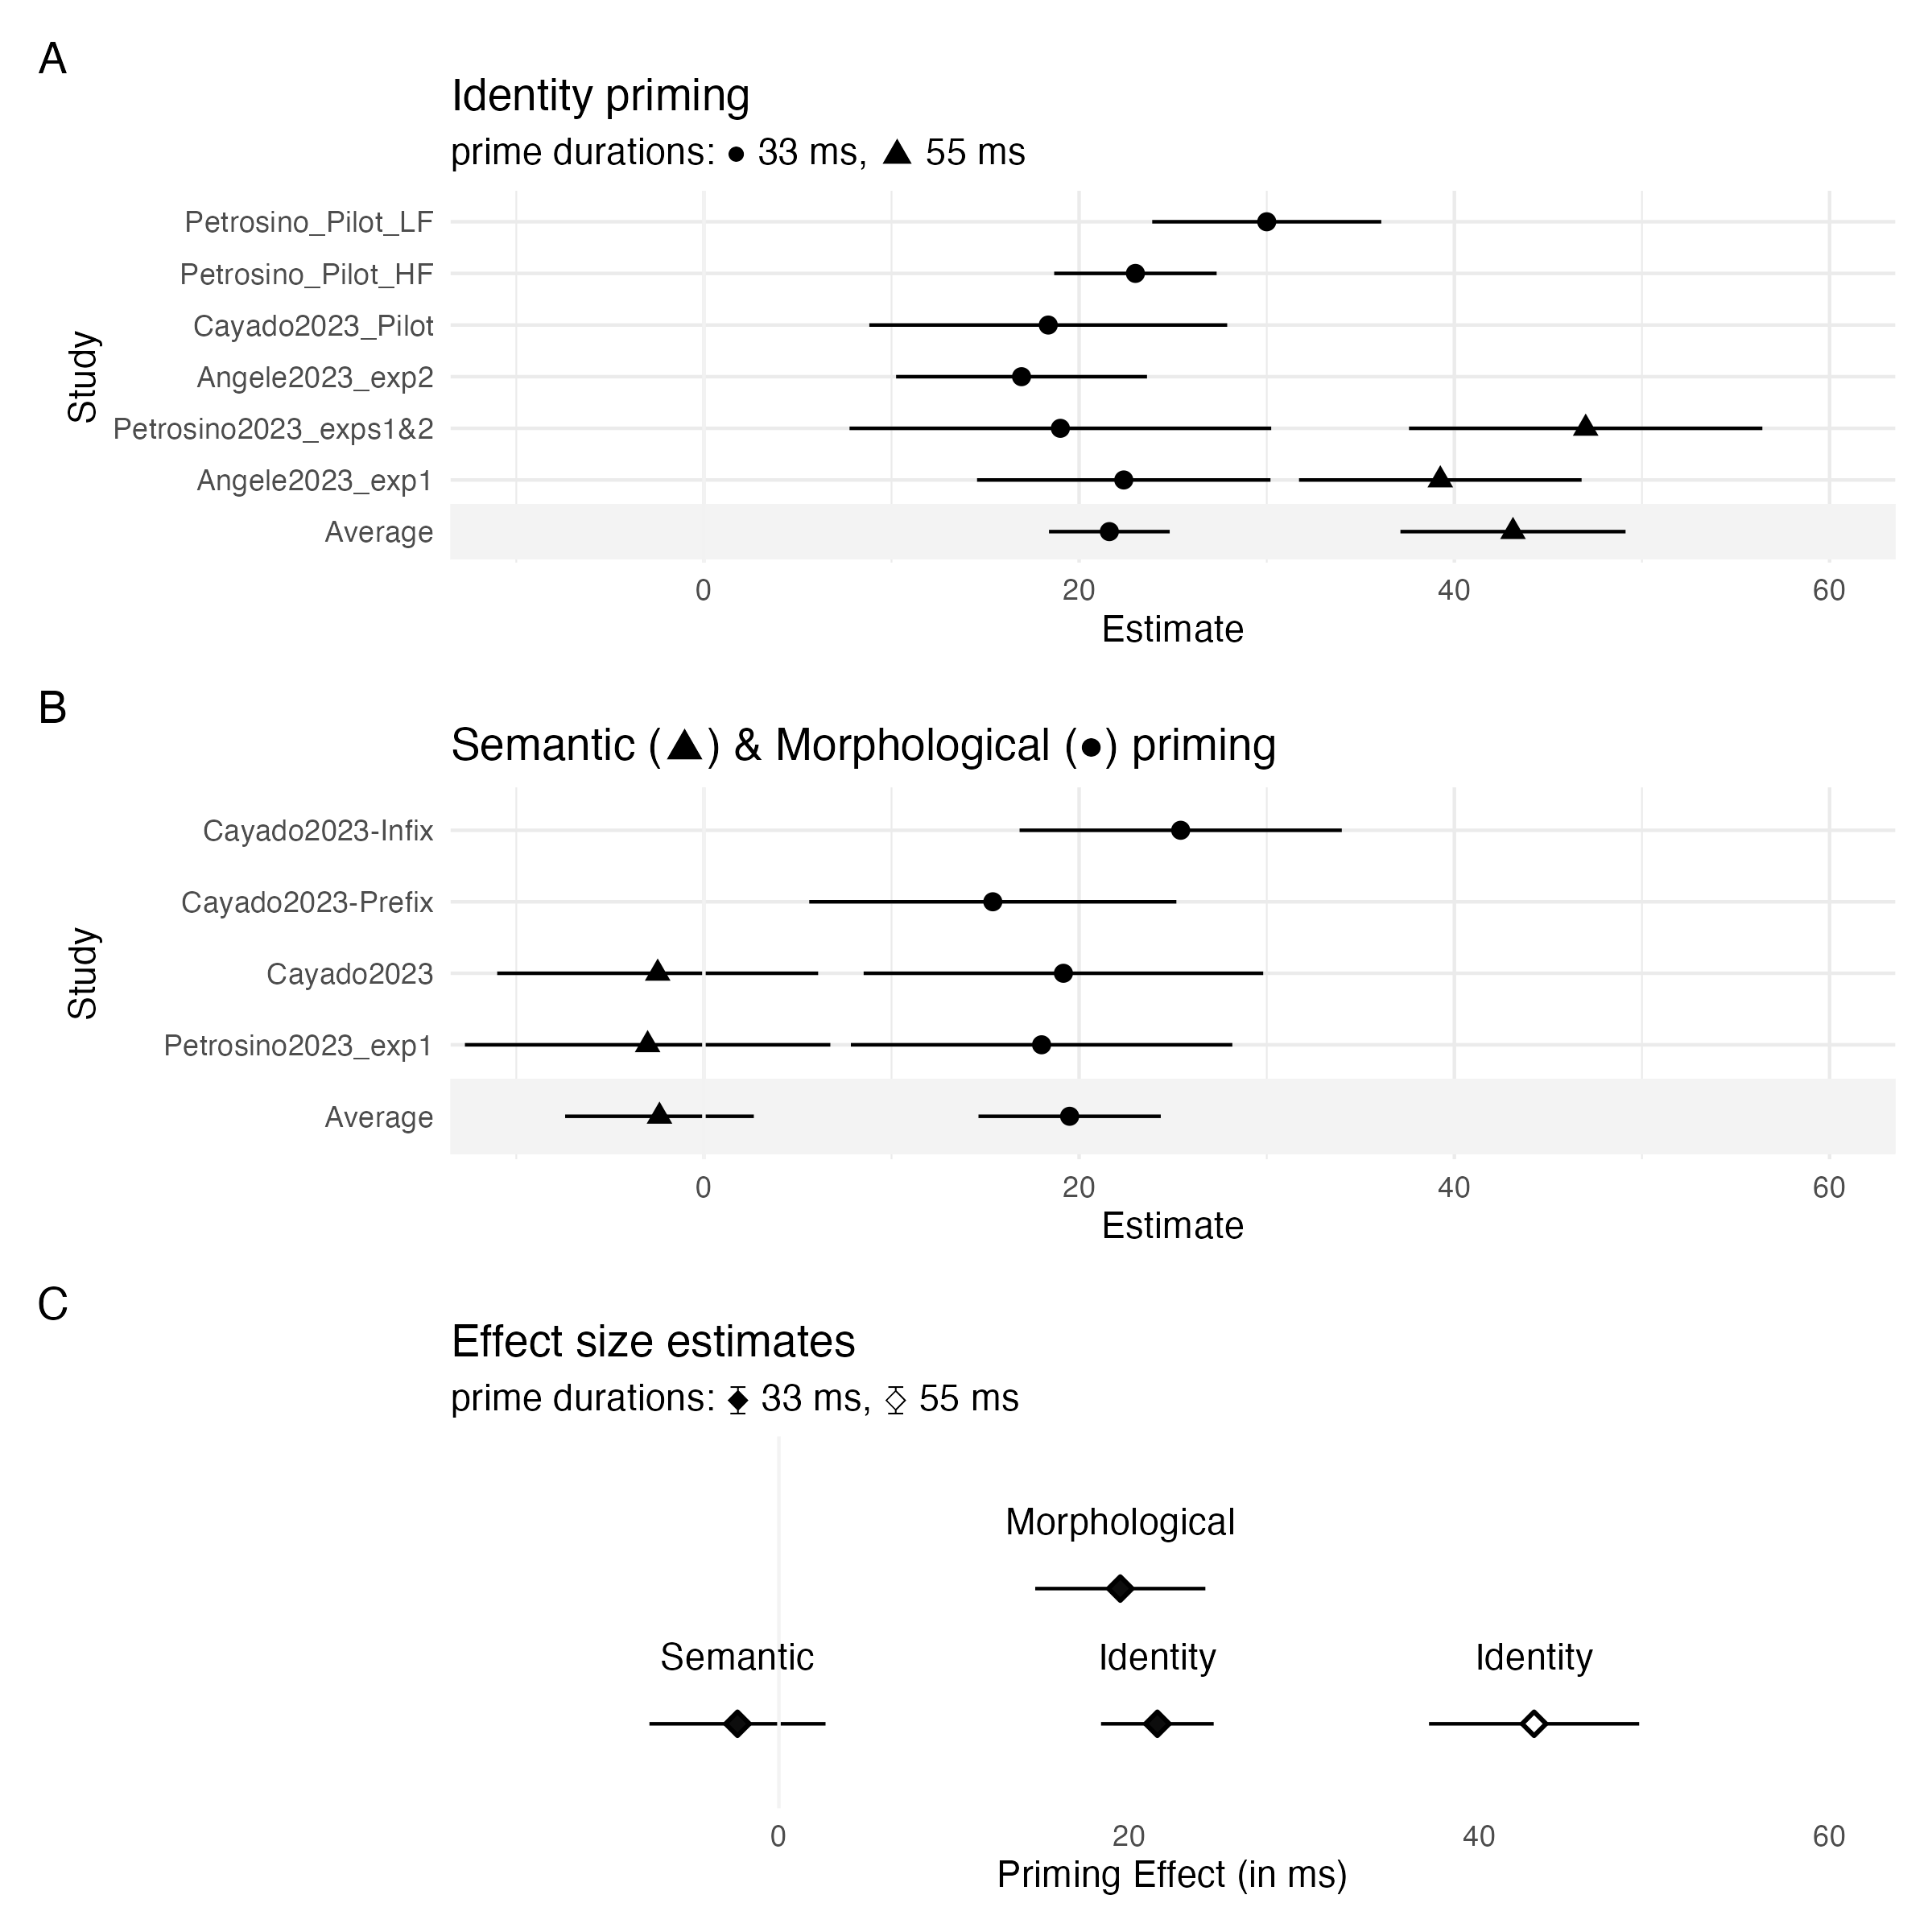
\includegraphics[keepaspectratio]{./supplemental-data/online_maskedpriming_meta.png}}

}

\caption{\label{fig-meta}Meta-analysis of three recent masked priming
experiments conducted online, together with unpublished pilot data from
our lab, investigating three different phenomena: identity,
morphological and semantic priming, at 33ms and 50ms prime durations.}

\end{figure}%

Notably, three recent studies have already demonstrated the viability of
conducting masked priming experiments online, employing different
software tools: Angele et al. (2023) with \emph{PsychoJS}, Cayado, Wray,
and Stockall (2023) with \emph{Gorilla} and Petrosino, Sprouse, and
Almeida (2023) with \emph{Labvanced}. Crucially, a meta-analysis (Bonett
2009) of their results (Figure~\ref{fig-meta}; the full details are
available in the supplemental material) show a clear replication of four
basic benchmark results in masked priming: detection of (i) identity and
(ii) morphological priming with (iii) no evidence of semantic priming,
as well as (iv) a proportionality effect of identity priming and prime
duration.

Building on these previous findings, experiment 1 attempts to determine
whether frequency attenuation effects can be observed under masked
priming. Experiment 2 focuses on whether frequency attenuation effects
may vary as a function of prime duration.

\section{Experiment 1}\label{sec-exp1}

Experiment 1 was designed to elicit a masked repetition priming response
to both high- and low-frequency words. The required sample size to
ensure adequate statistical power (\textgreater80\%) was determined
through a power analysis simulation (details and code available as
supplemental material at https://osf.io/r7d2q/). For a 10 ms FAE, a
sample size of 1,250 participants was identified as necessary to
maintain 80\% statistical power across a wide range of plausible
standard deviations and correlation structures between conditions. Given
the relatively untested nature of web browser-based masked priming
experiments, we opted for a larger sample size of 2,600 participants.
This decision was made to increase the likelihood of retaining at least
1,250 participants after applying exclusion criteria, while also
guaranteeing a narrow margin of error around the estimated effect size
(Maxwell, Kelley, and Rausch 2008).

The prime duration was set at 33 ms for three main reasons. First, prior
studies by Angele et al. (2023), Cayado, Wray, and Stockall (2023), and
Petrosino, Sprouse, and Almeida (2023) have demonstrated that a 33 ms
prime duration is sufficient to elicit reliable repetition priming
effects in web browser-based experiments. Second, this brief prime
duration ensures that the prime word is almost never consciously
perceived by participants (Forster, Mohan, and Hector 2003; Nievas
2010), providing a more accurate measure of early, presumably automatic
processes involved in word recognition. Lastly, previous research on the
\emph{Labvanced} platform (Petrosino, Sprouse, and Almeida 2023) has
shown that timing inaccuracies and missed screen refreshes can lead to
an increased number of trials with actual prime durations exceeding the
subliminal threshold (typically considered to be around 60 ms) when the
prime duration is set to 50 ms. If a significant number of trials exceed
the subliminal threshold, it may prompt participants to adopt
experiment-wide strategies, ultimately compromising the observed masked
priming response (Zimmerman and Gomez 2012).

\subsection{Methods}\label{sec-exp1-methods}

\subsubsection{Preregistration}\label{sec-exp1-prereg}

We preregistered the results of the power analysis, the goals, the
design and analysis plan for this experiment prior to data collection.
The preregistration is available online
(\url{https://doi.org/10.17605/OSF.IO/3NFQP}).

\subsubsection{Participants}\label{sec-exp1-methods-participants}

Two thousand and six hundred participants (1,445 females; \emph{mean
age} = 42, \emph{sd age} = 14) were recruited on Prolific
(\url{https://www.prolific.com}). Several criteria were selected to
ensure recruitment of native speakers of U.S. English: participants had
to be born in the Unites States of America, speak English as their first
and only language, and have no self-reported language-related disorder.
We encouraged participants to avoid any sort of distraction throughout
the experiment, and to close any program that may be running in the
background. However, because the experiment was run online, participants
could not be monitored during data collection. Finally, to further
reduce variability across participants' devices, we restricted the
experiment to be run on Google Chrome only, which at the time of this
writing is the most used browser worldwide (W3 Counter 2023), and
reportedly performs better than any other across operating systems (see
Lukács and Gartus 2023).

\subsubsection{Design}\label{sec-exp1-methods-design}

The masked priming procedure relied on a lexical decision task (LDT), in
which a 2 (frequency: \emph{high} vs \emph{low}) x 2 (prime type:
\emph{repetition} vs \emph{unrelated}) factorial design was used. Both
factors were manipulated within-subjects. The dependent variables were
lexical decision latency (RT, in milliseconds) and error rate (in
percentages).

\subsubsection{Materials}\label{sec-exp1-methods-materials}

One-hundred and four five-letter words, half of low frequency (between 7
and 24 occurrences per million in the SUBTLEX\(_{US}\) corpus) and half
of high frequency (between 57 and 2,961 occurrences per million in the
SUBTLEX\(_{US}\)) were sampled from the English Lexicon Project (Balota
et al. 2007). From each condition, 26 words were selected to be
presented as targets and related primes (the \emph{repetition}
condition), and the remaining 26 were presented as unrelated primes (the
\emph{unrelated} condition). All word items were also controlled for
orthographic neighborhood (i.e., Coltheart's \emph{N}): \(t \approx 0\).
All words used were monomorphemic nouns, adjectives, or verbs, thus
excluding particles, prepositions, and derived or inflected forms.

\begin{longtable}{lrrrrrrrrrrrrr}

\caption{\label{tbl-words_exp1}Experiment 1. Descriptive statistics of
the word items used. For both frequency databases, the word frequencies
were converted to per-million count to ensure cross-comparison.}

\tabularnewline

\toprule
 &  & \multicolumn{4}{c}{\textbf{HAL}} & \multicolumn{4}{c}{\textbf{SUBTLEX\textsubscript{US}}} & \multicolumn{4}{c}{\textbf{Orthographic \emph{N}}} \\ 
\cmidrule(lr){3-6} \cmidrule(lr){7-10} \cmidrule(lr){11-14}
frequency & N & min & max & mean & SD & min & max & mean & SD & min & max & mean & SD \\ 
\midrule\addlinespace[2.5pt]
high & 52 & 45 & 4984 & 573 & 808 & 57 & 2691 & 210 & 388 & 0 & 10 & 3.98 & 2.60 \\ 
low & 52 & 6 & 570 & 64 & 93 & 7 & 24 & 13 & 5 & 0 & 11 & 3.92 & 2.79 \\ 
\bottomrule

\end{longtable}

One-hundred and four five-letter, phono-orthographically legal non-words
were randomly selected from the English Lexicon Project database as
well. Half of them (i.e., 52) were randomly selected to be presented as
targets; the other half was instead used as unrelated non-word primes.
None of the non-words contained any existing English morpheme. Both the
words and non-words used in the experiments are reported in the appendix
at the end of the paper (after the References section). In addition, all
items had an error rate in the ELP smaller than 10\%, to ensure that
they would all be clearly distinguishable from words by participants.

\subsubsection{Procedure}\label{sec-exp1-methods-proc}

Each recruited participant was assigned one of two word lists, which
differed only in the relatedness of the prime with respect to the
target; otherwise, the two lists presented the same set of target words
and nonwords (i.e., 104 pairs for each list). In one list, the three
conditions (the high- and low-frequency word conditions, and the
non-word condition) had half of the target items being preceded by
themselves (the \emph{repetition} condition) and half of the target
items being preceded by one of the unrelated primes belonging to the
same frequency bin (the \emph{unrelated} condition). In the other list,
these assignments were reversed. The order of stimulus presentation was
randomized for each participant.

After being recruited in the \emph{Prolific} online platform,
participants were asked to click on a link redirecting them to the
Labvanced online service. During the experiment, they were asked to
perform a lexical decision task by pressing either the `J' (for word) or
`F' (for non-word) keys on their keyboard. Each trial consisted of three
different stimuli appearing at the center of the screen: a series of
five hashes (\#\#\#\#\#) presented for 500 ms, followed by a prime word
presented for 33 ms, and finally the target word; the target word
disappeared from the screen as soon as a decision was made.

Participants were given 5 breaks throughout the experiment. When the
experiment was over, the participants were then redirected to Prolific
in order to validate their submission. The median time to finish the
experiment was 6 minutes and participants were paid a rate of 9
GBP/hour.

\subsection{Data analysis}\label{sec-exp1-analysis}

Our preregistered data analysis plan established that the data would be
analyzed using a \textbf{\emph{2x3}} repeated factors ANOVA (condition,
3 levels: high vs.~low vs.~non-word; primetype, 2 levels: unrelated
vs.~repetition), with only subjects as random factors, followed by
planned comparisons between related and unrelated primetype for each
condition. The choice of this statistical model follows the
recommendations of Raaijmakers, Schrijnemakers, and Gremmen (1999) and
Raaijmakers (2003), and allowed us to carry out the power analysis
simulations that informed our sample size choice, since models that
include items as random factors or even as crossed random factors are
too computationally expensive to run in large scale statistical power
simulations. However, since these models have become more widely
adopted, we also present an analysis using Generalized Linear Mixed
Model (GLMM) analysis on the raw RT and the raw accuracy data. Unlike
linear mixed-effect models, GLMMs do not assume normal distribution of
the data, and are therefore particularly useful for non-normally
distributed data such as RTs and accuracy. For the RT data, a Gamma
distribution was used; for the accuracy data, a binomial distribution
was used instead. Both models used an identity link between fixed
effects and the dependent variable (Lo and Andrews 2015). To prevent
converge failure, the model was kept as simple as possible, with
\emph{condition}, \emph{primetype} and their interaction as fixed
effects. Subjects and items were crossed as random effects. Before
fitting the model, the contrasts were also set to sum-to-zero contrasts
(i.e., by using the R function \texttt{contr.sum()}) to facilitate
interpretation of main and interaction effects. The fitting was
performed by using the \texttt{lme4} R-package (Bates et al. 2015) with
the Laplace approximation technique, using 1 million iterations and the
BOBYQA optimizer to help convergence. The function \texttt{Anova()} from
the \texttt{car} R-package (Fox and Weisberg 2019) was used to obtain
estimates and probability values for fixed effects calculated for
Type-III sums of squares. Estimated marginal means were then calculated
with the function \texttt{emmeans()} from the the \texttt{emmeans}
R-package (Lenth 2024).

Analysis scripts and an abridged version of the data collected can be
found online (\url{https://osf.io/vn3r2}), and consisted of 297,598
observations in total. The pre-processing of the data consisted of three
separate steps.

\subsubsection{Step 1: subject and item
performance}\label{sec-exp1-analysis-performance}

Item and subject error rates were calculated. The item error rate was
never above 14\%, so no item was excluded from analysis. 19 subjects
were removed because their error rate was above 30\%. Thus, a total of
269,652 observations and 2,593 participants were included in further
analyses.

\subsubsection{Step 2: prime
durations}\label{sec-exp1-analysis-primeTime}

During the experiment, the duration of presentation of the prime word
was recorded for every trial. Both the mean (mean = 32 ms; sd=15 ms) and
the median (33 ms) of the prime duration confirm some imprecision in the
duration of the presentation of the prime during the experiment. This
was expected and likely due to the inherent difficulty with timing
precision of visual presentations in web browsers and the great
variation of computer hardware and internet connections used by the
participants. Both of these issues may be impossible to control, at
least at the current state of browser development. However, in masked
priming, in which the duration of the prime is an essential part of the
design, such fluctuations may indeed hinder proper elicitation of the
priming response. Thus, we only kept trials whose prime durations were
within a pre-set range from the intended prime duration of 33 ms. Taking
a standard 60-Hz monitor as reference, the lower and the upper bounds
were set respectively at 25 ms (i.e., the intended prime duration minus
half of a full refresh cycle: \(33-8~ ms\); noting that Angele et al.
(2023) already showed that no repetition priming effects are obtained
with a 16.7ms prime duration) and 60 ms (i.e., the commonly accepted
upper threshold of subliminal processing), in an attempt to remove any
trial that could have been consciously perceived by participants. This
cut-off removed 13 \% of the trials. No participant was excluded, for a
total of 237,287 observations.

\subsubsection{Step 3: RT analysis}\label{sec-exp1-analysis-RT}

After removing the incorrect responses, 0.51\% of the trials were
excluded if their corresponding RT was below 200 ms or above 1800 ms.
Finally, 249 subjects were removed because the number of trials within
the same condition was less than 7 (i.e., about half of the total number
of trials being presented within the same condition, i.e.~13). A total
of 210,889 observations and 2,341 subjects were included in the
statistical analysis below.

\subsection{Results}\label{sec-exp1-results}

Priming effects were calculated by subtracting the mean RT to the
related condition to the mean RT from the unrelated condition. We ran
two different analyses, for both RT and error data.

The preregistered 2x3 repeated-measures ANOVA (condition, 3 levels: high
vs.~low vs.~non-word; primetype, 2 levels: unrelated vs.~repetition) on
the by-subject averaged RT data revealed significant main effects
(condition: \emph{F}(1, 2340)=1572, \emph{p}\textless.0001; primetype:
\emph{F}(1, 2340)=1113, \emph{p}\textless.0001) and their interaction
\emph{F}(1, 2340)=52.48, \emph{p}\textless.0001). Planned comparisons
confirmed statistically significant repetition priming effects for both
word conditions (\emph{MOP\_HF}=18 ms, \emph{CI\_95\%}={[}16 20{]},
\emph{t}(2340)=19.7, \emph{p}\textless.0001; \emph{MOP\_LF} = 28 ms,
\emph{CI\_95\%}={[}26 30{]}, \emph{t}(2340)=27.8,
\emph{p}\textless.0001), with the low-frequency word repetition priming
effect being 10 ms larger than the high-frequency word repetition
priming effect. This FAE effect was statistically significant
(\emph{M\_FAE}=10 ms, \emph{CI\_95\%}={[}7 13{]}, \emph{t}(2340)=7.24,
\emph{p}\textless.0001). A very small, but statistically significant
inhibitory priming effect was observed in the non-word condition
(\emph{MOP\_NW}=-2 ms, \emph{CI\_95\%}={[}-4 0{]}, \emph{t}(2340)=-2.33,
\emph{p}\textless.0001). Similarly, the GLMM analysis confirmed that
both main effects (condition: \(\chi^2=2978.35, p<.0001\); primetype:
\(\chi^2=1531.12, p<.0001\)), and their interaction
(\(\chi^2=870.27, p<.0001\)) were significant. As reported in
Table~\ref{tbl-exp1-statsResults-anova} and
Table~\ref{tbl-exp1-statsResults-glmm}, the estimates based on the ANOVA
and GLMM models overlap with one another, which suggest the two models
to be substantially equivalent.

In the error analysis, the ANOVA revealed significant effects for both
main effects (condition: \emph{F}(1, 2340)=392.5,
\emph{p}\textless.0001; primetype: \emph{F}(1, 2340)=380.5,
\emph{p}\textless.0001) and interaction \emph{F}(1, 2340)=55.47,
\emph{p}\textless.0001). Planned comparisons revealed significant
priming effects in the form of fewer errors in the repeated compared to
unrelated trials in the all conditions (high: \emph{t}(2340)=9.95,
\emph{p}\textless.0001; low: \emph{t}(2340)=16.9,
\emph{p}\textless.0001; non-word: \emph{t}(2340)=-3.27, \emph{p}=.001).
As in the ANOVA error analysis, both main effects (condition:
\(\chi^2=30.45, p<.0001\); primetype: \(\chi^2=108.88, p<.0001\)) and
their interaction (\(\chi^2=307.57, p<.0001\)) were significant.

\blandscape

\begin{longtable}{lrrrrrrrrlrrrrl}

\caption{\label{tbl-exp1-statsResults-anova}Experiment 1. Summary of the
word priming results calculated within the ANOVA model. \emph{Legend.}
MOP: magnitude of priming.}

\tabularnewline

\toprule
 & \multicolumn{3}{c}{unrelated RT} & \multicolumn{3}{c}{repetition RT} &  & \multicolumn{4}{c}{priming effects} & \multicolumn{3}{c}{\emph{t}-test} \\ 
\cmidrule(lr){2-4} \cmidrule(lr){5-7} \cmidrule(lr){9-12} \cmidrule(lr){13-15}
factor & mean & SD & Error (\%) & mean & SD & Error (\%) & cor & MOP & 95\% CI & SD\textsubscript{p} & ES & \emph{t} & df & \emph{p} \\ 
\midrule\addlinespace[2.5pt]
high & 573 & 83 & 3 & 555 & 85 & 2 & 0.860 & 18 & [16 20] & 45 & 0.41 & 19.7 & 2340 & 2.88e-80 \\ 
low & 605 & 88 & 6 & 577 & 88 & 3 & 0.850 & 28 & [26 30] & 49 & 0.58 & 27.8 & 2340 & 1.52e-147 \\ 
non-word & 623 & 103 & 4 & 625 & 103 & 4 & 0.910 & -2 & [-4 0] & 43 & -0.05 & -2.33 & 2340 & 0.0197 \\ 
frequency:primetype &   &   &   &   &   &   & 0.029 & 10 & [7 13] & 66 & 0.15 & 7.24 & 2340 & 5.86e-13 \\ 
\bottomrule

\end{longtable}

\begin{longtable}{lrlrrlrrlr}

\caption{\label{tbl-exp1-statsResults-glmm}Experiment 1. Summary of the
word priming results calculated within the GLMM model. \emph{Legend.}
MOP: magnitude of priming.}

\tabularnewline

\toprule
 & \multicolumn{3}{c}{unrelated RT} & \multicolumn{3}{c}{repetition RT} & \multicolumn{3}{c}{priming effects} \\ 
\cmidrule(lr){2-4} \cmidrule(lr){5-7} \cmidrule(lr){8-10}
factor & mean & 95\% CI & SE & mean & 95\% CI & SE & MOP & 95\% CI & SE \\ 
\midrule\addlinespace[2.5pt]
high & 604 & [607 602] & 0.85 & 585 & [588 583] & 0.90 & 19 & [17 21] & 0.63 \\ 
low & 634 & [637 632] & 0.73 & 606 & [608 604] & 0.83 & 28 & [26 31] & 0.84 \\ 
non-word & 645 & [647 643] & 0.75 & 647 & [649 645] & 0.84 & -2 & [-4 0] & 0.62 \\ 
frequency*primetype &   &   &   &   &   &   & 9 & [7 12] & 1.03 \\ 
\bottomrule

\end{longtable}

\elandscape

\subsection{Discussion}\label{sec-exp1-discussion}

Experiment 1 was designed to investigate whether Frequency Attenuation
Effects (FAE) can be detected in masked priming with a prime duration of
33 ms. Our findings replicated the results of Angele et al. (2023),
Cayado, Wray, and Stockall (2023), and Petrosino, Sprouse, and Almeida
(2023), showing statistically significant masked repetition priming
effects in a web browser-based experiment for both high- and
low-frequency words. Crucially, the results also confirmed the presence
of an FAE, evidenced by a statistically significant interaction: the
priming effect for low-frequency words was 10 ms larger than that for
high-frequency words. Additionally, due to the large sample size, the
FAE was estimated with high precision, yielding a narrow margin of error
of 3 ms. Interestingly, in addition to the reliable FAE, our results
align with previous studies (Cayado, Wray, and Stockall 2023; Petrosino,
Sprouse, and Almeida 2023) in showing a minimal inhibitory masked
repetition priming effect for non-words, with very high precision. The
95\% confidence interval (CI) suggests that the plausible range for the
masked repetition priming effect for non-words, at a prime duration of
33 ms, is between -4 ms and 0 ms.

These findings help dispel doubts about whether an FAE can be observed
in masked priming, challenging earlier studies that failed to detect
this effect. However, the results also raise questions about the size
and malleability of the FAE. The FAE observed in Experiment 1 (10 ms) is
substantially smaller than those reported in other studies where
significant FAEs were found (e.g., Kinoshita 2006), where the effect was
around 30 ms. What could account for this discrepancy in effect size?
One possibility is that the 30 ms estimate is inflated due to the lower
statistical power in many previous experiments. As noted in the
introduction, low power can lead to overestimated effect sizes when
results are statistically significant. When examining the range of
effect sizes in Table~\ref{tbl-litReview}, we find that the average FAE
is approximately 15 ms, which is half the size of those observed when
statistically significant results were obtained. This 15 ms estimate is
closer to the 10 ms effect size observed in Experiment 1, but still
somewhat larger. Thus, there appears to be a potential discrepancy
between the FAE effect sizes reported in the literature and the estimate
from Experiment 1.

One possible explanation for this discrepancy is the difference in prime
duration used in Experiment 1 (33 ms) compared to most previous studies
(\(\geq 50 ms\)). It is plausible that the FAE scales linearly with
prime duration in masked priming, similar to how repetition priming
effects increase with longer prime durations. In fact, this is an actual
prediction of \emph{IA} models (see Grainger et al. 2012). Fortunately,
Angele et al. (2023) and Petrosino, Sprouse, and Almeida (2023) have
already demonstrated that web browser-based experiments can replicate
the proportionality between prime duration and the magnitude of masked
identity priming, consistent with Forster, Mohan, and Hector (2003).
Both studies showed that increasing the prime duration from 33 ms to 50
ms resulted in larger identity priming effects. This provides an
opportunity to test whether the discrepancy in FAE effect size between
Experiment 1 and prior literature is due to the shorter prime duration
used in our study. The goal of Experiment 2, therefore, is to leverage
the established linear scaling of repetition effects with prime duration
in masked priming to determine whether extending the prime duration also
increases the magnitude of the FAE.

\section{Experiment 2}\label{sec-exp2}

Experiment 2 is an exact replication of experiment 1, with one
difference: the prime duration is set to 50ms instead of 33ms. The
predictions are straightforward: if the FAE scales with prime duration,
then the FAE in experiment 2 should be larger than the one observed in
experiment 1. This result would explain why the FAE observed in
experiment 1 was smaller than the ones observed in prior studies.

In order to facilitate the interpretation of the results of experiment
2, we calculate the 95\% \emph{prediction intervals} (PI; cf. Patil,
Peng, and Leek 2016; Spence and Stanley 2016) for a replication of
experiment 1 with the effective sample size of experiment 2 (cf.
Table~\ref{tbl-pis}). The logic of the \emph{prediction interval} is to
establish a range of possible effect sizes that can be expected in a
replication due only to sampling error. In order words, if the only
difference between the original study and the replication study is
sampling variability, we should expect the effect sizes of the
replication study to fall within the 95\% PI set by the previous study.

According to Table~\ref{tbl-pis}, we can make the following predictions
for experiment 2: (1) Non-word repetition effects in masked priming are
thought to be independent of prime duration (mostly because they are at
best negligible to begin with). Thus, as far as the non-words are
concerned, experiment 2 can be seen as a simple replication of
experiment 1. The \emph{PI\_95\%} for non-words from experiment 1 is
{[}-5ms 1ms{]}. Thus, we expect that the effect size for non-word
repetition in experiment 2 could be as low a -5ms or as high as 1ms; any
result beyond these bounds would strongly imply that the differences
between the effect sizes of the two experiments cannot be explained
simply in terms of sampling error. (2) Masked repetition effects for
words, on the other hand, are thought to linearly increase in magnitude
as a function of prime duration. Thus, we expect that in experiment 2
the repetition effect size for LF and HF conditions should be superior
to the upper bounds of the \emph{PIs\_95\%} of experiment 1. The
\emph{PI\_95\%} from experiment 1 for the the repetition of HF words is
{[}15ms 21ms{]}; the one for the LF condition is {[}25ms 31ms{]}. Thus,
if our prime duration manipulation is successful in experiment 2, we
should expect the repetition effect for the HF condition to be larger
than 21ms while the same effect for the LF condition should be larger
than 31 ms. (3) It is presently unclear whether the FAE interacts with
prime duration. Given the FAE \emph{PI\_95\%} {[}6ms 14ms{]} from
experiment 1, we can interpret the results of experiment 2 in the
following manner: if the FAE in experiment 2 falls within the {[}6ms
14ms{]} interval, we have no particular reason to think that FAE
interacts with prime duration, as this result is exactly what would have
been predicted if experiment 2 was a direct replication of experiment 1.
However, if the FAE in experiment 2 is larger than 14 ms (as the
previous literature implies), then we have good reason to believe that
the FAE linearly scales with prime duration, much like masked repetition
priming effects do.

\begin{longtable}{lrrrrl}

\caption{\label{tbl-pis}Prediction intervals calculated on the means and
standard deviations (SD) of the conditions tested in experiment 1.}

\tabularnewline

\toprule
 &  &  & \multicolumn{2}{c}{sample size} &  \\ 
\cmidrule(lr){4-5}
factor & mean & SD & experiment 1 & experiment 2 & 95\% PI \\ 
\midrule\addlinespace[2.5pt]
high & 18 & 45 & 2341 & 1924 & [15 21] \\ 
low & 28 & 49 & 2341 & 1924 & [25 31] \\ 
non-word & -2 & 43 & 2341 & 1924 & [-5 1] \\ 
frequency:primetype & 10 & 66 & 2341 & 1924 & [6 14] \\ 
\bottomrule

\end{longtable}

\subsection{Methods}\label{sec-exp2-methods}

\subsubsection{Participants}\label{sec-exp2-methods-participants}

Two thousand and six hundred participants (1,551 females; \emph{mean
age} = 39, \emph{sd age} = 12) were recruited on Prolific
(\url{https://www.prolific.com}) with the same criteria specified for
experiment 1 (Section~\ref{sec-exp1-methods-participants}). Participants
from experiment 1 were excluded from the recruiment pool, to ensure an
completely new set of participants.

\subsubsection{Design}\label{sec-exp2-methods-design}

The experimental design was identical to experiment 1.

\subsubsection{Materials}\label{sec-exp2-methods-materials}

The experimental items were the same as experiment 1.

\subsubsection{Procedure}\label{sec-exp2-methods-proc}

Experiment 2 followed the same procedures as experiment 1 (see
Section~\ref{sec-exp1-methods-proc}). The only difference was the prime
duration, which was set to 50 ms. The median time to finish the
experiment was about 6 minutes, like in experiment 1.

\subsection{Data analysis}\label{sec-exp2-analysis}

The analysis and data pre-processing plan were the same as in experiment
1 (Section~\ref{sec-exp1-analysis}). Analysis scripts and an abridged
version of the data collected can be found online
(\url{https://osf.io/k3gpc}), and consisted of 295,940 observations in
total.

\subsubsection{Step 1: subject and item
performance}\label{sec-exp2-analysis-performance}

Item and subject error rates were calculated. Similarly to experiment 1,
the item error rate was never above 12\%, so no item was excluded from
analysis. 39 subjects were removed because their error rate was above
30\%. Thus, a total of 265,982 observations and 2,558 participants were
included in further analyses.

\subsubsection{Step 2: prime
durations}\label{sec-exp2-analysis-primeTime}

Prime fluctuations were dealt with in the same way as in experiment 1
(Section~\ref{sec-exp1-analysis-primeTime}). The mean (mean = 50.11 ms,
sd = 11.13 ms) and the median (median = 50 ms) prime durations were
closer to the intended value (50 ms). The same prime duration cut-off
set for experiment 1 (i.e., any trial whose prime duration was out of
the 25-60ms range) removed 20 \% of the trials. As compared to
experiment 1, experiment 2 had therefore a 7\% larger percentage of
removed out-of-range trials, the majority of which (18\%) were above the
subliminal threshold. This is in contrast with the distribution of the
prime durations in experiment 1, where the trials above the range
amounted to only 0\% of the dataset. As observed in previous studies and
pilot conducted in our lab, this distribution suggests that setting the
prime duration closer to either limit of a given range has the side
effect of allowing for more fluctuations beyond either limit, thus
potentially leading to greater data loss (see also further below). No
participant was excluded, for a total of 213,078 observations.

\subsubsection{Step 3: RT analysis}\label{sec-exp2-analysis-RT}

After removing the incorrect responses, similarly to experiment 1
(Section~\ref{sec-exp1-analysis-RT}), 0.59\% of the trials were excluded
if their corresponding RT was below 200 ms or above 1800 ms. Finally,
634 subjects were removed because the number of trials within the same
condition was less than 7 (i.e., about half of the total number of
trials being presented within the same condition, i.e.~13). A total of
168,195 observations and 1,924 subjects were included in the statistical
analysis below. The substantial number of subjects being removed at this
final stage was the side effect of the increased number of out-of-range
trials that were removed during the previous step of analysis,
demonstrating that setting the prime duration closer to the upper bound
of the subliminal range may incur in a higher degree of data loss in
online masked priming experiments.

\subsection{Results}\label{sec-exp2-results}

In the word analysis, the 2x3 repeated-measures ANOVA model revealed
significant main effects (condition: \emph{F}(1, 1923)=987.4,
\emph{p}\textless.0001; primetype: \emph{F}(1, 1923)=1447,
\emph{p}\textless.0001) and interaction \emph{F}(1, 1923)=36.82,
\emph{p}\textless.0001). Planned comparisons confirmed statistically
significant repetition priming effects for both word conditions
(\emph{MOP\_HF}=26 ms, \emph{CI\_95\%}={[}24 28{]}, \emph{t}(1923)=24.6,
\emph{p}\textless.0001; \emph{MOP\_LF} = 35 ms, \emph{CI\_95\%}={[}33
37{]}, \emph{t}(1923)=30.2, \emph{p}\textless.0001), with the
low-frequency word repetition priming effect being 10 ms larger than the
high-frequency word repetition priming effect. This FAE effect was
statistically significant (\emph{M\_FAE}=9 ms, \emph{CI\_95\%}={[}6
12{]}), \emph{t}(1920)=6.07, \emph{p}\textless.0001). A very small but
statistically significant inhibitory priming effect was observed in the
non-word condition (\emph{MOP\_NW}=-4 ms, \emph{CI\_95\%}={[}-6 -2{]},
\emph{t}(1923)=-3.53, \emph{p}=.0004). The GLMM analysis confirmed
significant effects for condition (\(\chi^2=2613.3, p<.0001\)),
primetype (\(\chi^2=1700.5, p<.0001\)), and their interaction
(\(\chi^2=1158.9, p<.0001\)). Similarly to experiment 1, the estimates
of both models were equivalent (see
Table~\ref{tbl-exp2-statsResults-anova} and
Table~\ref{tbl-exp2-statsResults-glmm})

In the error analysis, the ANOVA showed significant effects for both
main effects (condition: \emph{F}(1, 2340)=392.5,
\emph{p}\textless.0001; primetype: \emph{F}(1, 2340)=380.5,
\emph{p}\textless.0001) and interaction \emph{F}(1, 2340)=55.47,
\emph{p}\textless.0001). Planned comparisons confirmed significant
priming effects in the form of fewer errors in repeated compared to
unrelated trials in the all conditions (high: \emph{t}(1923)=9.30,
\emph{p}\textless.0001; low: \emph{t}(1923)=15.8,
\emph{p}\textless.0001; non-word: \emph{t}(1923)=-2.32, \emph{p}=.002).
Similar results were obtained in the GLMM error analysis (condition:
\(\chi^2=51.50, p<.0001\); primetype: \(\chi^2=97.42, p<.0001\);
interaction: \(\chi^2=283.77, p<.0001\)).

\blandscape

\begin{longtable}{lrrrrrrrrlrrrrr}

\caption{\label{tbl-exp2-statsResults-anova}Experiment 2. Summary of the
word priming results within the ANOVA model. \emph{Legend.} MOP:
magnitude of priming.}

\tabularnewline

\toprule
 & \multicolumn{3}{c}{unrelated RT} & \multicolumn{3}{c}{repetition RT} &  & \multicolumn{4}{c}{priming effects} & \multicolumn{3}{c}{\emph{t}-test} \\ 
\cmidrule(lr){2-4} \cmidrule(lr){5-7} \cmidrule(lr){9-12} \cmidrule(lr){13-15}
factor & mean & SD & Error (\%) & mean & SD & Error (\%) & cor & MOP & 95\% CI & SD\textsubscript{p} & ES & \emph{t} & df & \emph{p} \\ 
\midrule\addlinespace[2.5pt]
high & 574 & 83 & 3 & 548 & 83 & 2 & 0.850 & 26 & [24 28] & 46 & 0.56 & 24.595576 & 1923 & 2.27e-116 \\ 
low & 605 & 89 & 6 & 570 & 89 & 3 & 0.840 & 35 & [33 37] & 51 & 0.69 & 30.185474 & 1923 & 3.51e-164 \\ 
non-word & 629 & 108 & 4 & 633 & 110 & 5 & 0.900 & -4 & [-6 -2] & 50 & -0.08 & -3.525726 & 1923 & 4.32e-04 \\ 
frequency:primetype &   &   &   &   &   &   & 0.024 & 9 & [6 12] & 68 & 0.13 & 6.068254 & 1923 & 1.55e-09 \\ 
\bottomrule

\end{longtable}

\begin{longtable}{lrlrrlrrlr}

\caption{\label{tbl-exp2-statsResults-glmm}Experiment 2. Summary of the
word priming results within the GLMM model. \emph{Legend.} MOP:
magnitude of priming.}

\tabularnewline

\toprule
 & \multicolumn{3}{c}{unrelated RT} & \multicolumn{3}{c}{repetition RT} & \multicolumn{3}{c}{priming effects} \\ 
\cmidrule(lr){2-4} \cmidrule(lr){5-7} \cmidrule(lr){8-10}
factor & mean & 95\% CI & SE & mean & 95\% CI & SE & MOP & 95\% CI & SE \\ 
\midrule\addlinespace[2.5pt]
high & 605 & [608 603] & 0.81 & 579 & [582 577] & 0.87 & 26 & [24 28] & 0.80 \\ 
low & 633 & [635 631] & 0.81 & 598 & [600 596] & 0.77 & 35 & [32 37] & 0.85 \\ 
non-word & 649 & [652 647] & 0.95 & 653 & [655 650] & 0.96 & -3 & [-5 -1] & 0.73 \\ 
frequency*primetype &   &   &   &   &   &   & 8 & [6 11] & 1.05 \\ 
\bottomrule

\end{longtable}

\elandscape

\subsection{Discussion}\label{sec-exp2-discussion}

Experiment 2 aimed to replicate the FAE observed in Experiment 1 using
an extended prime duration of 50 ms, and to assess whether this longer
prime would amplify the effect. To achieve this, the same stimuli and
sample size from Experiment 1 were employed, with the sole modification
being the increased prime duration.

As predicted, we found that the masked repetition priming effect for
both high- and low-frequency words increased by approximately 8 ms in
Experiment 2 compared to Experiment 1. Specifically, the repetition
priming effect for high-frequency words was 26 ms, and for low-frequency
words, 35 ms, both exceeding the upper bounds of the 95\% prediction
interval from Experiment 1 (21 ms and 31 ms, respectively). This
indicates that the manipulation of prime duration was effective.
Notably, and consistent with our predictions, the repetition effect for
the non-word condition was -2 ms, which fell within the 95\% prediction
interval of Experiment 1 (i.e., {[}-5 1{]}). Furthermore, the larger
priming response for the high- and low-frequency word conditions in
Experiment 2 was driven entirely by faster recognition of the related
word pairs. The RT estimates for the unrelated pairs, along with their
standard deviations and error rates, were highly similar to those
observed in Experiment 1. This finding lends additional support to the
notion that the magnitude of the masked priming response is influenced
by prime duration (Forster, Mohan, and Hector 2003).

Crucially, we were also able to replicate the FAE in Experiment 2.
However, the FAE in this experiment was 9 ms
(\emph{CI\_95\%}\(_{exp2} = [6 12]\)), which is nearly identical to the
FAE observed in Experiment 1 and falls within its 95\% prediction
interval, i.e.~{[}6 ms 14 ms{]}. This suggests that, unlike the
repetition effect in masked priming, the FAE does not interact with
prime duration. Therefore, the difference in prime duration between
Experiment 1 and prior studies in the literature does not appear to
account for the observed discrepancies in the magnitude of the FAEs.

\section{General discussion}\label{sec-discussion}

The masked priming paradigm stands as a cornerstone in psycholinguistic
investigations, providing critical insights into the mechanisms of word
recognition. However, there is still uncertainty about whether lexical
frequency interacts with masked repetition priming, a phenomenon known
as the Frequency Attenuation Effect (FAE). Many early findings suggested
no such interaction, but more recent studies have contradicted this view
(see Table~\ref{tbl-litReview}). Resolving this issue is theoretically
important, as different word recognition models make divergent
predictions about whether the FAE should occur in masked priming, and,
if it does, how it should be explained.

\subsection{Accounting for the FAE}\label{accounting-for-the-fae}

On one side, \emph{interactive activation} (IA) models (McClelland and
Rumelhart 1981; Grainger and Jacobs 1996; Coltheart et al. 2001) and
\emph{retrospective models} of priming, such as the \emph{memory
recruitment model} (Bodner and Masson 1997; Masson and Bodner 2003;
Bodner and Masson 2014), predict the FAE in masked priming. However,
these theories differ in where they locate the effect. \emph{IA} models
predict a lexical origin (see Grainger et al. 2012), while the memory
recruitment model suggests a post-lexical source.

On the other side, \emph{search models}, such as the \emph{entry-opening
model} (Forster and Davis 1984), propose a more complex interaction
between lexical and episodic memory. These models posit that under
unmasked conditions, repetition priming is driven largely by
\emph{episodic} memory, but under masked priming, \emph{episodic} memory
plays no role, and thus masked repetition priming reveals primarily
\emph{lexical} (and perhaps also \emph{sublexical}) level processes.
According to the \emph{entry-opening model}, only two processes are at
play within lexical structure: a frequency-ordered lexical search and
the time required to open an entry once a potential match is flagged
(the \emph{entry opening time}, EOT). The search is sensitive to word
frequency, but the EOT is assumed to be uniform across all entries (and
it is estimated at roughly 60ms by Forster, Mohan, and Hector 2003).
Consequently, the model predicts no interaction between frequency and
repetition priming under masked conditions, meaning the FAE should not
be observable in masked repetition priming.

Clearly then, the FAE in experiments 1 and 2 empirically aligns with the
predictions of \emph{IA} and \emph{memory recruitment} models, insofar
as both models predict an FAE under masked conditions. These findings
contradict the \emph{entry opening model}, which predict predict no FAE
in masked repetition priming. However, further considerations suggest
that the FAEs observed in our studies may be less supportive of the
\emph{memory recruitment model}, which predicts the FAE only when the
context of the behavioral task justifies drawing on a non-lexical memory
resources post-lexically, such as increased task difficulty. In our
experiments, task difficulty was deliberately minimized: both words and
non-words had very high accuracy rates in the English Lexicon Project,
leading to item error rates that never rose above 14\%, entirely
avoiding the need for item exclusions. In addition, only 58 in 5200
participants, or 1.1\%, had an overall error rate above 30\%. Finally,
many researchers may find implausible the assumption that episodic
memory resources are formed at the very short prime duration used in
experiment 1 (33 ms). Conversely, the \emph{entry-opening model}
predicts a null FAE because it assumes a fixed EOT. This assumption,
based on the observation that the magnitude of masked repetition effects
mirror prime duration up to 60 ms (Forster, Mohan, and Hector 2003), is
contradicted by our findings. In Experiment 2, where the prime duration
was 50 ms, the maximum repetition priming effect was 35 ms for
low-frequency words, suggesting that EOTs are not fixed at 60 ms, nor do
they match the prime duration in general (see Wu 2012 for a similar
argument). Moreover, repetition priming effects were consistently
smaller for high-frequency words, further challenging the model's
assumption of uniform EOTs. Thus, if we relax the assumption that EOTs
are uniform across the lexicon and instead posit that lower-frequency
words have longer entry opening times than higher-frequency words, the
\emph{entry-opening model}, like \emph{IA} models, could account for the
FAE.

\subsection{The independence of FAE from prime
duration}\label{the-independence-of-fae-from-prime-duration}

What about the finding that the FAE does not seem to interact with prime
duration? Here, these models seem to make the wrong predictions.
\emph{IA} models assume that it is stimulus exposure that drives
activation of lexical nodes, and that frequency is directly related with
lexical nodes activation levels, either in terms of setting their
resting levels or in how fast they accumulate information from the
input. Grainger et al. (2012) explains how the FAE is predicted by such
a model: low-frequency words accumulate evidence more slowly that do
high-frequency words. If one posits that stimulus repetition provide a
uniform boost to lexical nodes, then compared to a situation where
lexical nodes are at their resting activation levels (the unrelated
condition), lower-frequency repeated words will reach their recognition
threshold comparatively faster than would repeated high-frequency words
(cf. Grainger et al. 2012, fig. 1). Under this view, however, the amount
of activation boost to lexical nodes in the related condition is a
function of stimulus exposure, and thus a longer prime duration should
deliver a stronger initial activation boost, which can only lead to a
magnification of the FAE. Therefore, it seems that the basic mechanics
of \emph{IA} models, together with the assumptions that allow them to
capture the FAE, also predict an interactive effect between FAE
magnitude and prime duration, with larger FAE magnitudes predicted when
prime durations are longer. In experiments 1 and 2, however, the
increase from a 33ms to a 50ms prime duration elicited FAEs of same
magnitude (approximately 10ms).

The original \emph{entry opening model} does not predict a FAE, and so
it cannot make any predictions about its potential interaction with
prime duration. However, the modified version of the \emph{entry opening
model} sketched above would be able to. If it is indeed true that EOTs
are larger for lower-frequency words, then the relationship between
prime duration and FAE should be somewhat non-linear: while prime
duration equals the EOTs of the higher frequency words, then no FAE
should be observed. While the prime duration exceeds the EOTs for the
higher frequency words, but it is still shorter than the EOTs of the
lower frequency words, the FAE should increase linearly with prime
duration. It should reach its maximum when the prime duration equals the
EOTs of the lower frequency words. Beyond that point, increases in prime
duration should no longer lead to increases in FAE, which should remain
at its maximum magnitude, namely the difference between the EOTs of
high- and low-frequency words.

Unfortunately, we do not observe this predicted pattern in experiments 1
and 2. For instance, in Experiment 1, the repetition effect for
low-frequency words is close to the prime duration (a 28ms effect for a
33ms prime duration), while the repetition effect for high-frequency
words is 10ms shorter (a 18ms effect for a 33ms prime duration). If we
assume that 28ms is not significantly different from 33ms, the modified
\emph{entry opening model} would predict that the prime duration has not
yet exceeded the \emph{opening times} of the low frequency words, while
it clearly has exceeded the \emph{opening times} of the high-frequency
words. Thus, the model would predict that an increase in prime duration
would also increase the magnitude of the repetition effect for the LF
condition, but not for the HF condition, leading to a larger FAE.
However, while we did observe an increase in the magnitude of the
repetition effect for the LF condition in experiment 2 (28ms in Exp.1
and 35ms in Exp.2), the same was true for the HF condition (18ms in
Exp.1 and 26ms in Exp.2), and thus the FAE was identical in magnitude
across experiments. Conversely, if we take the results of experiment 1
at face value, and assume that the 33ms prime duration exceeds both the
\emph{opening times} of high- and low-frequency words (18ms and 28ms
respectively), then the modified \emph{entry opening model} would indeed
make the prediction that the FAE observed in experiment 1 reveals the
maximum of the FAE as 10ms, and that this value should not increase when
prime duration increases. However, the same model would also make the
prediction that the repetition priming effects should remain stable
across experiments, contrary to fact (they are both approximately 8ms
longer in experiment 2).

Thus, it seems neither \emph{IA} models nor the modified \emph{entry
opening model} make the correct predictions about the pattern of results
observed in experiments 1 and 2, namely a stable FAE effect across
increases in prime duration, with a concomitant increase in repetition
priming effects as a function of prime duration. \emph{IA} models would
have predicted an increased FAE in experiment 2, and the modified
\emph{entry opening model} would have predicted either an increased FAE
in experiment 2, or exactly identical results in terms of FAE and
repetition priming effects magnitudes in experiments 1 and 2.

Can these models be amended to allow them to capture the results? On the
one hand, given their core mechanics, \emph{IA} models can capture
either a situation where FAE does not arise (ie. frequency is purely
additive to repetition effects), or a situation where FAE is generated
and its magnitude is necessarily a function of the prime duration.
Neither of these patterns match the results of experiments 1 and 2. So
the results of experiment 1 and 2 pose a real challenge for \emph{IA}
models.

On the other hand, a different modification to the original \emph{entry
opening model} may help explain both the existence of the FAE and its
non-interaction with prime duration. If we assume that the exposure to
the prime raises the rank order of the target word to the top of the
search list, this would result in a boost that is a simple function of
the repeated presentation, and therefore should not interact with prime
duration. This boost would also impact high- and low-frequency words
differently: while both words would benefit from repetition by being
raised to the top of the search list, low-frequency words would be
retrieved comparatively faster than high-frequency words when contrasted
with their first retrieval times during the presentation of the prime.
This simple mechanism explains at once the existence of the FAE and the
fact that it does not interact with prime duration. For instance, in
experiment 1, the 10ms FAE can be explained as follows: as the EOT is
uniform, then it must be around 18ms (the repetition priming effect of
high-frequency words). The repetition priming effect for low-frequency
words (28ms) is then the the summation of the EOT (18ms) and the
comparative speed up difference in retrieval time for the target words
across high- and low-frequency condition (i.e, the FAE, which with this
set of materials is 10ms). Unfortunately, this logic would fail to
account for the results of experiment 2: if the EOT is indeed 18ms as
shown in experiment 1, and the EOT is the only source of priming for
high-frequency words, then this effect is already maxed out with a prime
duration of 33ms. Why is it then that increasing the prime duration to
50ms in experiment 2 makes the effect approximately 8ms longer (26ms)?
The only way this could be true is if the EOTs can vary substantially
across samples of individuals; for instance, if the EOT for the sample
in experiment 1 was 18ms, but it was 26ms for the sample in experiment
2. The problem with this assumption is that it seems arbitrary to assume
that the EOT can vary substantially (here \textasciitilde8ms) across our
two very large samples, which are able to produce very narrow margins of
errors around precise estimates for a number of relevant measurements,
such as the mean and standard deviations RT for the unrelated conditions
and non-word conditions and the magnitude of the FAE. Nonetheless, it
may be a fruitful avenue for future studies to explore.

\section{Conclusion}\label{conclusion}

Our study successfully replicated and expanded upon the work of Angele
et al. (2023), Cayado, Wray, and Stockall (2023) and Petrosino, Sprouse,
and Almeida (2023), confirming the viability of observing repetition
priming effects in masked priming experiments conducted online with both
a short (33ms) and longer (50ms) priming durations. Notably, we were
able to successfully address a lingering empirical question in the
literature by establishing that the Frequency Attenuation Effect (FAE)
does arises under masked conditions. We were able to determine
additionally that the FAE is also independent of the duration of the
prime. We contend that, while this pattern of results presents a direct
challenge to both \emph{IA} and \emph{entry opening} models, the latter
offers a few promising avenues for small modifications might enable it
to accommodate the results of our studies. The most promising is the
assumption that after the encounter with the prime, its entry is
temporarily raised to the top of the rank frequency ordered search list.
This modification explains at once the existence of the FAE, and its
independence of the prime duration.

\newpage{}

\section*{References}\label{references}
\addcontentsline{toc}{section}{References}

\phantomsection\label{refs}
\begin{CSLReferences}{1}{0}
\bibitem[\citeproctext]{ref-Adelman2014}
Adelman, James S, Rebecca L Johnson, Samantha F McCormick, Meredith
McKague, Sachiko Kinoshita, Jeffrey S Bowers, Jason R Perry, et al.
2014. {``A Behavioral Database for Masked Form Priming.''}
\emph{Behavior Research Methods} 46: 1052--67.

\bibitem[\citeproctext]{ref-Angele2023}
Angele, Bernhard, Ana Baciero, Pablo Gómez, and Manuel Perea. 2023.
{``Does Online Masked Priming Pass the Test? The Effects of Prime
Exposure Duration on Masked Identity Priming.''} \emph{Behavior Research
Methods} 55 (1): 151--67.
\url{https://doi.org/10.3758/s13428-021-01742-y}.

\bibitem[\citeproctext]{ref-Anwyl2020}
Anwyl-Irvine, Alexander L, Jessica Massonnié, Adam Flitton, Natasha
Kirkham, and Jo K Evershed. 2020. {``Gorilla in Our Midst: An Online
Behavioral Experiment Builder.''} \emph{Behavior Research Methods} 52:
388--407.

\bibitem[\citeproctext]{ref-Balota2004}
Balota, David A., Michael J. Cortese, Susan D. Sergent-Marshall, Daniel
H. Spieler, and Melvin J. Yap. 2004. {``Visual Word Recognition of
Single-Syllable Words.''} \emph{Journal of Experimental Psychology:
General} 133 (2): 283.

\bibitem[\citeproctext]{ref-balota2007}
Balota, David A., Melvin J. Yap, Keith A. Hutchison, Michael J. Cortese,
Brett Kessler, Bjorn Loftis, James H. Neely, Douglas L. Nelson, Greg B.
Simpson, and Rebecca Treiman. 2007. {``The English Lexicon Project.''}
\emph{Behavior Research Methods} 39 (3): 445--59.
\url{https://doi.org/10.3758/bf03193014}.

\bibitem[\citeproctext]{ref-BatesEtal2015}
Bates, Douglas, Reinhold Kliegl, Shravan Vasishth, and Harald Baayen.
2015. {``Parsimonious Mixed Models.''}
\url{https://arxiv.org/abs/1506.04967}.

\bibitem[\citeproctext]{ref-Bodner2014}
Bodner, Glen E., and Michael E. J Masson. 2014. {``Memory Recruitment: A
Backward Idea about Masked Priming.''} In \emph{Psychology of Learning
and Motivation}, 61:179--213. Elsevier.

\bibitem[\citeproctext]{ref-BodnerMasson1997}
Bodner, Glen E., and Michael E. J. Masson. 1997. {``Masked Repetition
Priming of Words and Nonwords: Evidence for a Nonlexical Basis for
Priming.''} \emph{Journal of Memory and Language} 37 (2): 268--93.
\url{https://doi.org/10.1006/jmla.1996.2507}.

\bibitem[\citeproctext]{ref-BodnerMasson2001}
---------. 2001. {``Prime Validity Affects Masked Repetition Priming:
Evidence for an Episodic Resource Account of Priming.''} \emph{Journal
of Memory and Language} 45 (4): 616--47.
\url{https://doi.org/10.1006/jmla.2001.2791}.

\bibitem[\citeproctext]{ref-Bonett2009}
Bonett, Douglas G. 2009. {``Meta-Analytic Interval Estimation for
Standardized and Unstandardized Mean Differences.''} \emph{Psychological
Methods} 14 (3): 225.

\bibitem[\citeproctext]{ref-Brysbaert2011}
Brysbaert, Marc, and Michael J Cortese. 2011. {``Do the Effects of
Subjective Frequency and Age of Acquisition Survive Better Word
Frequency Norms?''} \emph{Quarterly Journal of Experimental Psychology}
64 (3): 545--59.

\bibitem[\citeproctext]{ref-Brysbaert2018}
Brysbaert, Marc, Paweł Mandera, and Emmanuel Keuleers. 2018. {``The Word
Frequency Effect in Word Processing: An Updated Review.''} \emph{Current
Directions in Psychological Science} 27 (1): 45--50.

\bibitem[\citeproctext]{ref-BrysbaertNew2009}
Brysbaert, Marc, and Boris New. 2009. {``Moving Beyond Ku{č}era and
Francis: A Critical Evaluation of Current Word Frequency Norms and the
Introduction of a New and Improved Word Frequency Measure for American
English.''} \emph{Behavior Research Methods} 41 (4): 977--90.
\url{https://doi.org/10.3758/brm.41.4.977}.

\bibitem[\citeproctext]{ref-BrysbaertStevens2018}
Brysbaert, Marc, and Michaël Stevens. 2018. {``Power Analysis and Effect
Size in Mixed Effects Models: A Tutorial.''} \emph{Journal of Cognition}
1 (1). \url{https://doi.org/10.5334/joc.10}.

\bibitem[\citeproctext]{ref-Burgess1998}
Burgess, Curt, and Kay Livesay. 1998. {``The Effect of Corpus Size in
Predicting Reaction Time in a Basic Word Recognition Task: Moving on
from Ku{č}era and Francis.''} \emph{Behavior Research Methods,
Instruments, \& Computers} 30 (2): 272--77.

\bibitem[\citeproctext]{ref-Button2013}
Button, Katherine S, John PA Ioannidis, Claire Mokrysz, Brian A Nosek,
Jonathan Flint, Emma SJ Robinson, and Marcus R Munafò. 2013. {``Power
Failure: Why Small Sample Size Undermines the Reliability of
Neuroscience.''} \emph{Nature Reviews Neuroscience} 14 (5): 365--76.

\bibitem[\citeproctext]{ref-Cayado2023}
Cayado, Dave Kenneth Tayao, Samantha Wray, and Linnaea Stockall. 2023.
{``Does Linear Position Matter for Morphological Processing? Evidence
from a Tagalog Masked Priming Experiment.''} \emph{Language, Cognition
and Neuroscience}, 1--16.

\bibitem[\citeproctext]{ref-Cohen1992}
Cohen, Jacob. 1992. {``A Power Primer.''} \emph{Psychological Bulletin}
112 (1): 155--59. \url{https://doi.org/10.1037/0033-2909.112.1.155}.

\bibitem[\citeproctext]{ref-ColtheartEtal2001}
Coltheart, Max, Kathleen Rastle, Conrad Perry, Robyn Langdon, and
Johannes Ziegler. 2001. {``DRC: A Dual Route Cascaded Model of Visual
Word Recognition and Reading Aloud.''} \emph{Psychological Review} 108
(1): 204--56.

\bibitem[\citeproctext]{ref-deLeeuw2014}
de Leeuw, Joshua R. 2014. {``jsPsych: A JavaScript Library for Creating
Behavioral Experiments in a Web Browser.''} \emph{Behavior Research
Methods} 47 (1): 1--12. \url{https://doi.org/10.3758/s13428-014-0458-y}.

\bibitem[\citeproctext]{ref-EvettHumphreys1981}
Evett, Lindsay J., and Glyn W. Humphreys. 1981. {``The Use of Abstract
Graphemic Information in Lexical Access.''} \emph{The Quarterly Journal
of Experimental Psychology} 33 (4): 325--50.

\bibitem[\citeproctext]{ref-Labvanced2017}
Finger, Holger, Caspar Goeke, Dorena Diekamp, Kai Standvoß, and Peter
König. 2017. {``LabVanced: A Unified JavaScript Framework for Online
Studies.''} In \emph{2017 International Conference on Computational
Social Science}. Cologne, Germany.

\bibitem[\citeproctext]{ref-Forster1998}
Forster, Kenneth I. 1998. {``The Pros and Cons of Masked Priming.''}
\emph{Journal of Psycholinguistic Research} 27 (2): 203--33.

\bibitem[\citeproctext]{ref-ForsterDavis1984}
Forster, Kenneth I., and Chris Davis. 1984. {``Repetition Priming and
Frequency Attenuation in Lexical Access.''} \emph{Journal of
Experimental Psychology: Learning, Memory, and Cognition} 10 (4): 680.

\bibitem[\citeproctext]{ref-ForsterDavis1991}
Forster, Kenneth I., and Christopher Davis. 1991. {``The Density
Constraint on Form-Priming in the Naming Task: Interference Effects from
a Masked Prime.''} \emph{Journal of Memory and Language} 30 (1): 1--25.
\url{https://doi.org/10.1016/0749-596x(91)90008-8}.

\bibitem[\citeproctext]{ref-ForsterEtal1987}
Forster, Kenneth I., C. Davis, C. Schoknecht, and R. Carter. 1987.
{``Masked Priming with Graphemically Related Forms: Repetition or
Partial Activation?''} \emph{The Quarterly Journal of Experimental
Psychology Section A} 39 (2): 211--51.
\url{https://doi.org/10.1080/14640748708401785}.

\bibitem[\citeproctext]{ref-ForsterEtal2003}
Forster, Kenneth I., Kathleen Mohan, and Jo Hector. 2003. {``The
Mechanics of Masked Priming.''} In \emph{Masked Priming: The State of
the Art}, edited by Sachiko Kinoshita and Stephen J. Lupker, 3--37. New
York, NY/Hove, UK: Psychology Press.

\bibitem[\citeproctext]{ref-FoxWeisberg2019}
Fox, John, and Sanford Weisberg. 2019. \emph{An {R} Companion to Applied
Regression}. Third. Thousand Oaks {CA}: Sage.
\url{https://socialsciences.mcmaster.ca/jfox/Books/Companion/}.

\bibitem[\citeproctext]{ref-GelmanCarlin2014}
Gelman, Andrew, and John Carlin. 2014. {``Beyond Power Calculations.''}
\emph{Perspectives on Psychological Science} 9 (6): 641--51.
\url{https://doi.org/10.1177/1745691614551642}.

\bibitem[\citeproctext]{ref-Gimenes2016}
Gimenes, Manuel, and Boris New. 2016. {``Worldlex: Twitter and Blog Word
Frequencies for 66 Languages.''} \emph{Behavior Research Methods} 48:
963--72.

\bibitem[\citeproctext]{ref-GraingerJacobs1996}
Grainger, Jonathan, and Arthur M. Jacobs. 1996. {``Orthographic
Processing in Visual Word Recognition: A Multiple Read-Out Model.''}
\emph{Psychological Review} 103 (3): 518.

\bibitem[\citeproctext]{ref-GraingerEtal2012}
Grainger, Jonathan, Danielle Lopez, Marianna Eddy, Stéphane Dufau, and
Phillip J Holcomb. 2012. {``How Word Frequency Modulates Masked
Repetition Priming: An ERP Investigation.''} \emph{Psychophysiology} 49
(5): 604--16.

\bibitem[\citeproctext]{ref-Herdaugdelen2017}
Herdağdelen, Amaç, and Marco Marelli. 2017. {``Social Media and Language
Processing: How Facebook and Twitter Provide the Best Frequency
Estimates for Studying Word Recognition.''} \emph{Cognitive Science} 41
(4): 976--95.

\bibitem[\citeproctext]{ref-Jacoby1983}
Jacoby, Larry L. 1983. {``Remembering the Data: Analyzing Interactive
Processes in Reading.''} \emph{Journal of Verbal Learning and Verbal
Behavior} 22 (5): 485--508.

\bibitem[\citeproctext]{ref-Jacoby1981}
Jacoby, Larry L, and Mark Dallas. 1981. {``On the Relationship Between
Autobiographical Memory and Perceptual Learning.''} \emph{Journal of
Experimental Psychology: General} 110 (3): 306.

\bibitem[\citeproctext]{ref-Kinoshita2006}
Kinoshita, Sachiko. 2006. {``Additive and Interactive Effects of Word
Frequency and Masked Repetition in the Lexical Decision Task.''}
\emph{Psychonomic Bulletin \& Review} 13 (4): 668--73.
\url{https://doi.org/10.3758/bf03193979}.

\bibitem[\citeproctext]{ref-KuceraFrancis1967}
Kučera, J., and W. N. Francis. 1967. \emph{Computational Analysis of
Present Day American English}. Providence, RI: Brown University Press.

\bibitem[\citeproctext]{ref-Lenth2024}
Lenth, Russell V. 2024. \emph{Emmeans: Estimated Marginal Means, Aka
Least-Squares Means}. \url{https://rvlenth.github.io/emmeans/}.

\bibitem[\citeproctext]{ref-LoAndrews2015}
Lo, Steson, and Sally Andrews. 2015. {``To Transform or Not to
Transform: Using Generalized Linear Mixed Models to Analyse Reaction
Time Data.''} \emph{Frontiers in Psychology} 6: 1171.

\bibitem[\citeproctext]{ref-LukacsGaspar2023}
Lukács, Gáspár, and Andreas Gartus. 2023. {``Precise Display Time
Measurement in JavaScript for Web-Based Experiments.''} \emph{Behavior
Research Methods} 55 (3): 1079--93.
\url{https://doi.org/10.3758/s13428-022-01835-2}.

\bibitem[\citeproctext]{ref-MassonBodner2003}
Masson, Michael E. J., and Glen E. Bodner. 2003. {``A Retrospective View
of Masked Priming: Toward a Unified Account of Masked and Long-Term
Repetition Priming.''} \emph{Masked Priming: The State of the Art},
57--94.

\bibitem[\citeproctext]{ref-Maxwell2008}
Maxwell, Scott E, Ken Kelley, and Joseph R Rausch. 2008. {``Sample Size
Planning for Statistical Power and Accuracy in Parameter Estimation.''}
\emph{Annu. Rev. Psychol.} 59 (1): 537--63.

\bibitem[\citeproctext]{ref-McClellandRumelhart1981}
McClelland, James L., and David E. Rumelhart. 1981. {``An Interactive
Activation Model of Context Effects in Letter Perception: Part i. An
Account of Basic Findings.''} \emph{Psychological Review} 88 (5):
375--407.

\bibitem[\citeproctext]{ref-Nievas2010}
Nievas, Francisco. 2010. {``The Frequency Attenuation Effect in Identity
and Associative Priming.''} \emph{The Spanish Journal of Psychology} 13
(1): 30--62. \url{https://doi.org/10.1017/s1138741600003668}.

\bibitem[\citeproctext]{ref-NorrisKinoshita2008}
Norris, Dennis, and Sachiko Kinoshita. 2008. {``Perception as Evidence
Accumulation and Bayesian Inference: Insights from Masked Priming.''}
\emph{Journal of Experimental Psychology: General} 137 (3): 434--55.
\url{https://doi.org/10.1037/a0012799}.

\bibitem[\citeproctext]{ref-Norris2018}
Norris, Dennis, Sachiko Kinoshita, Jane Hall, and Richard Henson. 2018.
{``Is Reading Automatic? Are the ERP Correlates of Masked Priming Really
Lexical?''} \emph{Language, Cognition and Neuroscience} 33 (9):
1152--67.

\bibitem[\citeproctext]{ref-Patil2016}
Patil, Prasad, Roger D Peng, and Jeffrey T Leek. 2016. {``What Should
Researchers Expect When They Replicate Studies? A Statistical View of
Replicability in Psychological Science.''} \emph{Perspectives on
Psychological Science} 11 (4): 539--44.

\bibitem[\citeproctext]{ref-PeirceEtal2019}
Peirce, Jonathan, Jeremy R. Gray, Sol Simpson, Michael MacAskill,
Richard Höchenberger, Hiroyuki Sogo, Erik Kastman, and Jonas Kristoffer
Lindeløv. 2019. {``PsychoPy2: Experiments in Behavior Made Easy.''}
\emph{Behavior Research Methods} 51 (1): 195--203.

\bibitem[\citeproctext]{ref-PetrosinoEtal2023}
Petrosino, Roberto, Jon Sprouse, and Diogo Almeida. 2023. {``Asymmetries
in the Stem and Suffix Masked Priming Response in a Large-Scale Online
Study.''} \emph{Quaderni Di Linguistica e Studi Orientali}, no. 49:
177--94. \url{https://doi.org/10.13128/QUL-SO-2421-7220-15154}.

\bibitem[\citeproctext]{ref-PotvinSchtuz2000}
Potvin, Patrick J., and Robert W. Schutz. 2000. {``Statistical Power for
the Two-Factor Repeated Measures ANOVA.''} \emph{Behavior Research
Methods, Instruments, \& Computers} 32 (2): 347--56.
\url{https://doi.org/10.3758/bf03207805}.

\bibitem[\citeproctext]{ref-Raaijmakers2003}
Raaijmakers, Jeroen GW. 2003. {``A Further Look at the"
Language-as-Fixed-Effect Fallacy".''} \emph{Canadian Journal of
Experimental Psychology/Revue Canadienne de Psychologie Exp{é}rimentale}
57 (3): 141.

\bibitem[\citeproctext]{ref-Raaijmakers1999}
Raaijmakers, Jeroen GW, Joseph MC Schrijnemakers, and Frans Gremmen.
1999. {``How to Deal with {`the Language-as-Fixed-Effect Fallacy'}:
Common Misconceptions and Alternative Solutions.''} \emph{Journal of
Memory and Language} 41 (3): 416--26.

\bibitem[\citeproctext]{ref-RajaramNeely1992}
Rajaram, Suparna, and James H Neely. 1992. {``Dissociative Masked
Repetition Priming and Word Frequency Effects in Lexical Decision and
Episodic Recognition Tasks.''} \emph{Journal of Memory and Language} 31
(2): 152--82. \url{https://doi.org/10.1016/0749-596x(92)90009-m}.

\bibitem[\citeproctext]{ref-ScarboroughEtal1977}
Scarborough, Don L., Charles Cortese, and Hollis S. Scarborough. 1977.
{``Frequency and Repetition Effects in Lexical Memory.''} \emph{Journal
of Experimental Psychology: Human Perception and Performance} 3 (1):
1--17. \url{https://doi.org/10.1037/0096-1523.3.1.1}.

\bibitem[\citeproctext]{ref-SeguiGrainger1990}
Segui, Juan, and Jonathan Grainger. 1990. {``Priming Word Recognition
with Orthographic Neighbors: Effects of Relative Prime-Target
Frequency.''} \emph{Journal of Experimental Psychology: Human Perception
and Performance} 16 (1): 65--76.
\url{https://doi.org/10.1037/0096-1523.16.1.65}.

\bibitem[\citeproctext]{ref-Sereno1991}
Sereno, Joan A. 1991. {``Graphemic, Associative, and Syntactic Priming
Effects at a Brief Stimulus Onset Asynchrony in Lexical Decision and
Naming.''} \emph{Journal of Experimental Psychology: Learning, Memory,
and Cognition} 17 (3): 459--77.
\url{https://doi.org/10.1037/0278-7393.17.3.459}.

\bibitem[\citeproctext]{ref-SpenceStanley2016}
Spence, Jeffrey R, and David J Stanley. 2016. {``Prediction Interval:
What to Expect When You're Expecting\ldots{} a Replication.''}
\emph{PloS One} 11 (9): 1--22.
\url{https://doi.org/10.1371/journal.pone.0162874}.

\bibitem[\citeproctext]{ref-w3counterGlobalStats}
W3 Counter. 2023. {``Browser \& Platform Market Share - November
2023.''}
\url{https://www.w3counter.com/globalstats.php?year=2023&month=11}.

\bibitem[\citeproctext]{ref-Wu2012}
Wu, Hongmei. 2012. {``Mechanisms of Masked Priming: Testing the Entry
Opening Model.''} PhD thesis, The University of Arizona.

\bibitem[\citeproctext]{ref-Yap2009}
Yap, Melvin J., and David A. Balota. 2009. {``Visual Word Recognition of
Multisyllabic Words.''} \emph{Journal of Memory and Language} 60 (4):
502--29.

\bibitem[\citeproctext]{ref-Zevin2002}
Zevin, Jason D, and Mark S Seidenberg. 2002. {``Age of Acquisition
Effects in Word Reading and Other Tasks.''} \emph{Journal of Memory and
Language} 47 (1): 1--29.

\bibitem[\citeproctext]{ref-Zimmerman2012}
Zimmerman, Robert, and Pablo Gomez. 2012. {``Drawing Attention to Primes
Increases Inhibitory Word Priming Effects.''} \emph{The Mental Lexicon}
7 (2): 119--46.

\end{CSLReferences}

\newpage{}

\section*{Wordlists}\label{wordlists}
\addcontentsline{toc}{section}{Wordlists}

\subsection*{Experiment 1}\label{experiment-1}
\addcontentsline{toc}{subsection}{Experiment 1}

\begin{longtable*}{lllrrrr}
\toprule
 &  &  & \multicolumn{2}{c}{RT (to repetition)} & \multicolumn{2}{c}{RT (to unrelated)} \\ 
\cmidrule(lr){4-5} \cmidrule(lr){6-7}
related & unrelated prime & word & mean & SD & mean & SD \\ 
\midrule\addlinespace[2.5pt]
\multicolumn{7}{l}{\emph{low frequency condition}} \\ 
\midrule\addlinespace[2.5pt]
arrow & hunch & arrow & 590 & 130 & 587 & 124 \\ 
pitch & sneak & pitch & 576 & 126 & 612 & 122 \\ 
hatch & widow & hatch & 621 & 151 & 639 & 148 \\ 
shark & brief & shark & 573 & 125 & 590 & 138 \\ 
tooth & sharp & tooth & 536 & 125 & 565 & 116 \\ 
booth & grief & booth & 572 & 136 & 627 & 157 \\ 
pound & sting & pound & 551 & 127 & 572 & 127 \\ 
weigh & thief & weigh & 593 & 167 & 636 & 164 \\ 
blank & avoid & blank & 571 & 139 & 596 & 124 \\ 
crush & award & crush & 554 & 128 & 592 & 136 \\ 
bench & smack & bench & 573 & 132 & 601 & 129 \\ 
fetch & brand & fetch & 622 & 156 & 658 & 146 \\ 
cheek & salad & cheek & 561 & 141 & 602 & 142 \\ 
brush & swamp & brush & 564 & 130 & 600 & 128 \\ 
march & depth & march & 559 & 125 & 580 & 123 \\ 
bleed & flesh & bleed & 560 & 148 & 577 & 146 \\ 
cliff & harsh & cliff & 602 & 130 & 645 & 137 \\ 
fraud & creep & fraud & 621 & 147 & 628 & 132 \\ 
cloud & plead & cloud & 536 & 115 & 551 & 101 \\ 
fluid & thumb & fluid & 605 & 140 & 678 & 162 \\ 
trash & creek & trash & 554 & 127 & 560 & 128 \\ 
flush & blond & flush & 576 & 123 & 617 & 140 \\ 
porch & stink & porch & 587 & 136 & 620 & 160 \\ 
stiff & patch & stiff & 626 & 154 & 678 & 156 \\ 
cough & sweep & cough & 564 & 142 & 601 & 141 \\ 
smash & squad & smash & 570 & 129 & 587 & 126 \\ 
\midrule\addlinespace[2.5pt]
\multicolumn{7}{l}{\emph{high frequency condition}} \\ 
\midrule\addlinespace[2.5pt]
blood & chief & blood & 541 & 130 & 551 & 104 \\ 
bunch & child & bunch & 585 & 148 & 617 & 145 \\ 
catch & board & catch & 545 & 116 & 562 & 130 \\ 
stuff & tough & stuff & 555 & 119 & 585 & 137 \\ 
break & stand & break & 545 & 107 & 561 & 124 \\ 
speak & beach & speak & 545 & 131 & 573 & 129 \\ 
stick & hotel & stick & 562 & 128 & 598 & 138 \\ 
sleep & angel & sleep & 538 & 113 & 559 & 119 \\ 
wrong & truth & wrong & 563 & 143 & 565 & 132 \\ 
grand & quick & grand & 571 & 127 & 582 & 143 \\ 
mouth & world & mouth & 543 & 125 & 556 & 119 \\ 
knock & extra & knock & 560 & 134 & 631 & 136 \\ 
guard & think & guard & 580 & 132 & 590 & 134 \\ 
small & thing & small & 557 & 130 & 577 & 125 \\ 
check & round & check & 558 & 135 & 562 & 121 \\ 
watch & proud & watch & 541 & 128 & 546 & 110 \\ 
group & smell & group & 559 & 127 & 576 & 142 \\ 
month & earth & month & 555 & 120 & 572 & 123 \\ 
south & relax & south & 575 & 139 & 611 & 133 \\ 
lunch & truck & lunch & 547 & 119 & 557 & 125 \\ 
clock & throw & clock & 548 & 132 & 574 & 124 \\ 
sound & death & sound & 538 & 127 & 552 & 103 \\ 
drink & north & drink & 559 & 129 & 556 & 122 \\ 
touch & young & touch & 541 & 122 & 573 & 121 \\ 
laugh & weird & laugh & 546 & 119 & 568 & 121 \\ 
black & reach & black & 553 & 131 & 563 & 114 \\ 
\midrule\addlinespace[2.5pt]
\multicolumn{7}{l}{non-word} \\ 
\midrule\addlinespace[2.5pt]
alkew & grack & alkew & 599 & 153 & 591 & 140 \\ 
agink & furob & agink & 626 & 148 & 614 & 141 \\ 
ruzak & begro & ruzak & 577 & 130 & 584 & 142 \\ 
sondo & labok & sondo & 625 & 142 & 612 & 149 \\ 
guesh & gazzo & guesh & 702 & 184 & 721 & 194 \\ 
fadio & criam & fadio & 618 & 149 & 604 & 146 \\ 
plich & coreb & plich & 650 & 162 & 640 & 159 \\ 
sgrew & docab & sgrew & 626 & 182 & 638 & 182 \\ 
sceak & colob & sceak & 675 & 154 & 683 & 171 \\ 
ghisk & isloo & ghisk & 588 & 139 & 593 & 139 \\ 
deirm & ahuck & deirm & 589 & 142 & 596 & 139 \\ 
villo & flurb & villo & 632 & 182 & 615 & 181 \\ 
tidow & pikto & tidow & 648 & 167 & 624 & 160 \\ 
drick & aliom & drick & 684 & 168 & 681 & 172 \\ 
phick & purso & phick & 643 & 160 & 637 & 165 \\ 
nello & borno & nello & 625 & 156 & 612 & 151 \\ 
feach & pacaw & feach & 730 & 201 & 720 & 192 \\ 
tello & rilth & tello & 651 & 175 & 644 & 171 \\ 
dolio & caveb & dolio & 602 & 148 & 610 & 165 \\ 
gorgo & swysh & gorgo & 643 & 164 & 619 & 170 \\ 
whilo & lanjo & whilo & 612 & 137 & 604 & 150 \\ 
stanf & drief & stanf & 611 & 134 & 617 & 133 \\ 
crulk & ocheb & crulk & 671 & 162 & 665 & 169 \\ 
phumb & tunch & phumb & 645 & 160 & 633 & 148 \\ 
sirth & steaf & sirth & 612 & 141 & 618 & 145 \\ 
slerk & nohew & slerk & 640 & 153 & 634 & 163 \\ 
vitbo & nualm & vitbo & 593 & 151 & 596 & 154 \\ 
sunch & ofium & sunch & 665 & 165 & 665 & 161 \\ 
soeth & croik & soeth & 589 & 141 & 589 & 130 \\ 
eltow & valuo & eltow & 628 & 171 & 606 & 158 \\ 
framo & sorgo & framo & 617 & 146 & 618 & 146 \\ 
lumpo & shavo & lumpo & 630 & 162 & 635 & 172 \\ 
spuff & oceab & spuff & 672 & 169 & 667 & 183 \\ 
gatob & tolio & gatob & 599 & 139 & 606 & 155 \\ 
nosom & theck & nosom & 598 & 155 & 604 & 139 \\ 
gezzo & tooch & gezzo & 592 & 136 & 586 & 131 \\ 
afoub & slonk & afoub & 582 & 133 & 589 & 128 \\ 
wateb & salch & wateb & 633 & 151 & 619 & 133 \\ 
nelch & raceb & nelch & 601 & 144 & 594 & 145 \\ 
dahoo & ahack & dahoo & 598 & 132 & 595 & 146 \\ 
driek & fideo & driek & 606 & 145 & 606 & 143 \\ 
gnask & fluko & gnask & 612 & 171 & 604 & 153 \\ 
brosk & cyrrh & brosk & 629 & 159 & 647 & 175 \\ 
duvez & revuo & duvez & 580 & 152 & 580 & 155 \\ 
fielm & cempo & fielm & 609 & 146 & 611 & 151 \\ 
pumph & exulk & pumph & 669 & 162 & 685 & 176 \\ 
gerif & kleck & gerif & 584 & 137 & 588 & 149 \\ 
racef & bonth & racef & 618 & 151 & 622 & 156 \\ 
pheek & scook & pheek & 640 & 155 & 644 & 176 \\ 
pruaw & slork & pruaw & 593 & 133 & 592 & 135 \\ 
guilm & whilf & guilm & 603 & 142 & 598 & 142 \\ 
lairf & drosh & lairf & 587 & 144 & 600 & 150 \\ 
\bottomrule
\end{longtable*}

\subsection*{Experiment 2}\label{experiment-2}
\addcontentsline{toc}{subsection}{Experiment 2}

\begin{longtable*}{lllrrrr}
\toprule
 &  &  & \multicolumn{2}{c}{RT (to repetition)} & \multicolumn{2}{c}{RT (to unrelated)} \\ 
\cmidrule(lr){4-5} \cmidrule(lr){6-7}
related & unrelated prime & word & mean & SD & mean & SD \\ 
\midrule\addlinespace[2.5pt]
\multicolumn{7}{l}{\emph{low frequency condition}} \\ 
\midrule\addlinespace[2.5pt]
arrow & hunch & arrow & 573 & 130 & 591 & 128 \\ 
pitch & sneak & pitch & 565 & 132 & 608 & 146 \\ 
hatch & widow & hatch & 606 & 163 & 644 & 164 \\ 
shark & brief & shark & 560 & 132 & 587 & 124 \\ 
tooth & sharp & tooth & 533 & 126 & 560 & 111 \\ 
booth & grief & booth & 566 & 147 & 618 & 163 \\ 
pound & sting & pound & 552 & 139 & 570 & 134 \\ 
weigh & thief & weigh & 583 & 158 & 649 & 186 \\ 
blank & avoid & blank & 556 & 132 & 583 & 132 \\ 
crush & award & crush & 542 & 126 & 583 & 142 \\ 
bench & smack & bench & 565 & 143 & 601 & 138 \\ 
fetch & brand & fetch & 612 & 149 & 663 & 146 \\ 
cheek & salad & cheek & 556 & 138 & 597 & 148 \\ 
brush & swamp & brush & 559 & 136 & 593 & 125 \\ 
march & depth & march & 560 & 149 & 575 & 122 \\ 
bleed & flesh & bleed & 552 & 137 & 568 & 135 \\ 
cliff & harsh & cliff & 595 & 149 & 662 & 157 \\ 
fraud & creep & fraud & 596 & 131 & 634 & 113 \\ 
cloud & plead & cloud & 539 & 132 & 552 & 108 \\ 
fluid & thumb & fluid & 601 & 167 & 690 & 173 \\ 
trash & creek & trash & 564 & 157 & 566 & 126 \\ 
flush & blond & flush & 570 & 133 & 624 & 155 \\ 
porch & stink & porch & 584 & 155 & 617 & 153 \\ 
stiff & patch & stiff & 617 & 163 & 677 & 161 \\ 
cough & sweep & cough & 552 & 136 & 591 & 145 \\ 
smash & squad & smash & 553 & 133 & 590 & 142 \\ 
\midrule\addlinespace[2.5pt]
\multicolumn{7}{l}{\emph{high frequency condition}} \\ 
\midrule\addlinespace[2.5pt]
blood & chief & blood & 534 & 131 & 558 & 112 \\ 
bunch & child & bunch & 584 & 156 & 619 & 146 \\ 
catch & board & catch & 529 & 111 & 568 & 141 \\ 
stuff & tough & stuff & 556 & 128 & 576 & 133 \\ 
break & stand & break & 542 & 128 & 564 & 123 \\ 
speak & beach & speak & 543 & 131 & 570 & 132 \\ 
stick & hotel & stick & 556 & 136 & 599 & 130 \\ 
sleep & angel & sleep & 525 & 111 & 566 & 137 \\ 
wrong & truth & wrong & 555 & 142 & 569 & 137 \\ 
grand & quick & grand & 564 & 129 & 588 & 147 \\ 
mouth & world & mouth & 534 & 123 & 552 & 116 \\ 
knock & extra & knock & 549 & 131 & 615 & 139 \\ 
guard & think & guard & 565 & 118 & 590 & 118 \\ 
small & thing & small & 549 & 137 & 567 & 130 \\ 
check & round & check & 546 & 125 & 563 & 120 \\ 
watch & proud & watch & 531 & 115 & 545 & 133 \\ 
group & smell & group & 553 & 126 & 579 & 142 \\ 
month & earth & month & 549 & 126 & 576 & 128 \\ 
south & relax & south & 563 & 138 & 603 & 144 \\ 
lunch & truck & lunch & 549 & 141 & 563 & 124 \\ 
clock & throw & clock & 547 & 133 & 574 & 130 \\ 
sound & death & sound & 534 & 127 & 559 & 147 \\ 
drink & north & drink & 550 & 124 & 563 & 116 \\ 
touch & young & touch & 545 & 145 & 567 & 120 \\ 
laugh & weird & laugh & 535 & 113 & 556 & 114 \\ 
black & reach & black & 547 & 129 & 578 & 129 \\ 
\midrule\addlinespace[2.5pt]
\multicolumn{7}{l}{non-word} \\ 
\midrule\addlinespace[2.5pt]
alkew & grack & alkew & 603 & 150 & 606 & 160 \\ 
agink & furob & agink & 632 & 161 & 615 & 155 \\ 
ruzak & begro & ruzak & 580 & 149 & 582 & 155 \\ 
sondo & labok & sondo & 619 & 168 & 621 & 178 \\ 
guesh & gazzo & guesh & 707 & 189 & 748 & 195 \\ 
fadio & criam & fadio & 632 & 169 & 602 & 171 \\ 
plich & coreb & plich & 645 & 148 & 646 & 180 \\ 
sgrew & docab & sgrew & 637 & 197 & 648 & 184 \\ 
sceak & colob & sceak & 692 & 179 & 692 & 165 \\ 
ghisk & isloo & ghisk & 595 & 149 & 594 & 152 \\ 
deirm & ahuck & deirm & 599 & 147 & 595 & 147 \\ 
villo & flurb & villo & 637 & 210 & 615 & 178 \\ 
tidow & pikto & tidow & 651 & 175 & 641 & 177 \\ 
drick & aliom & drick & 696 & 194 & 685 & 186 \\ 
phick & purso & phick & 648 & 176 & 639 & 168 \\ 
nello & borno & nello & 631 & 178 & 637 & 189 \\ 
feach & pacaw & feach & 748 & 201 & 745 & 208 \\ 
tello & rilth & tello & 665 & 185 & 662 & 174 \\ 
dolio & caveb & dolio & 618 & 175 & 609 & 157 \\ 
gorgo & swysh & gorgo & 651 & 179 & 631 & 178 \\ 
whilo & lanjo & whilo & 619 & 150 & 615 & 164 \\ 
stanf & drief & stanf & 613 & 147 & 627 & 134 \\ 
crulk & ocheb & crulk & 678 & 173 & 679 & 183 \\ 
phumb & tunch & phumb & 655 & 175 & 648 & 180 \\ 
sirth & steaf & sirth & 623 & 146 & 616 & 136 \\ 
slerk & nohew & slerk & 644 & 167 & 638 & 172 \\ 
vitbo & nualm & vitbo & 590 & 143 & 596 & 154 \\ 
sunch & ofium & sunch & 664 & 162 & 676 & 172 \\ 
soeth & croik & soeth & 590 & 131 & 589 & 146 \\ 
eltow & valuo & eltow & 638 & 170 & 603 & 153 \\ 
framo & sorgo & framo & 626 & 165 & 631 & 162 \\ 
lumpo & shavo & lumpo & 634 & 172 & 635 & 164 \\ 
spuff & oceab & spuff & 683 & 182 & 665 & 204 \\ 
gatob & tolio & gatob & 607 & 167 & 594 & 154 \\ 
nosom & theck & nosom & 603 & 156 & 608 & 160 \\ 
gezzo & tooch & gezzo & 601 & 160 & 600 & 164 \\ 
afoub & slonk & afoub & 583 & 136 & 587 & 133 \\ 
wateb & salch & wateb & 640 & 159 & 641 & 160 \\ 
nelch & raceb & nelch & 609 & 163 & 595 & 145 \\ 
dahoo & ahack & dahoo & 611 & 157 & 597 & 154 \\ 
driek & fideo & driek & 613 & 152 & 610 & 151 \\ 
gnask & fluko & gnask & 606 & 154 & 606 & 159 \\ 
brosk & cyrrh & brosk & 637 & 165 & 649 & 180 \\ 
duvez & revuo & duvez & 590 & 168 & 576 & 154 \\ 
fielm & cempo & fielm & 621 & 181 & 614 & 160 \\ 
pumph & exulk & pumph & 687 & 184 & 697 & 202 \\ 
gerif & kleck & gerif & 587 & 154 & 586 & 147 \\ 
racef & bonth & racef & 619 & 164 & 621 & 151 \\ 
pheek & scook & pheek & 641 & 157 & 635 & 169 \\ 
pruaw & slork & pruaw & 599 & 157 & 598 & 143 \\ 
guilm & whilf & guilm & 620 & 168 & 603 & 163 \\ 
lairf & drosh & lairf & 590 & 138 & 597 & 146 \\ 
\bottomrule
\end{longtable*}




\end{document}
